\documentclass{mcmthesis}
\mcmsetup{CTeX = false,
        tcn = 12519, problem = Using Land: A Valuable Resource,
        sheet = true, titleinsheet = false, keywordsinsheet = false,
        titlepage = false, abstract = false}
\setlength{\headheight}{13.6pt}
\usepackage{newtxtext}%\usepackage{times}
%to get dummy loremipsum text
\usepackage{lipsum}
\usepackage{subcaption}
\usepackage{booktabs}
\usepackage{minted}
\usepackage{amsmath}
\usepackage{blkarray}
\usepackage{caption}
\usepackage{nicematrix}
\usepackage{longtable}
\usepackage{xltabular}
\usepackage{graphicx}
\usepackage{algorithm2e}
\RestyleAlgo{ruled}
\usepackage{pdfpages}
\usepackage[numbib,nottoc]{tocbibind}


\usepackage[svgnames]{xcolor}
%for unknown reason, including the following packages changes the style of the contents section
% \usepackage{multicol}
% \usepackage{tocloft}
% \usepackage{titletoc}
\title{IMMC Challenge}
\date{\today}
\begin{document}
\begin{abstract}
How do land developers decide what to build? In a small town near Syracuse, New York, there is a roughly 3-square-kilometer plot of land being considered for the development of a new business. The local "decision-makers" need help determining the best use of land given several business options, such as sports facilities and various types of farms. To help them decide, we designed a quantitative metric to define the "best" use of the land.

As a part of the problem, we were provided with the land characteristics and specific location of the plot. Additionally, we were instructed to assume that the plot of land has adequate water, power supplies, and soil that is sufficiently rich for crop farming or grazing animals. 

To begin, we determined the most significant characteristics affecting land developers' decisions, leading us to divide the decision process into three main factors: (a) project feasibility, (b) long-term environmental conditions, and (c) economic potential. By evaluating these factors alongside individualized importance rankings, we were able to create a model that allows the decision-makers to balance community values and business profits in their final decision. 

To determine the project's feasibility, our model considers usable surface area, average changes in elevation, and proximity to local bodies of water. Next, we used predictive modeling to anticipate the future conditions of the land, ensuring that our decision model is viable in the long run. Finally, we evaluated economic potential using financial indicators that account for profitability and community interests for each business option. 

Since the decision-makers are willing to divide the property into different sections, we utilized the sliding-window method, which applies our decision-making process to multiple sizes of "windows" or subplots. Specifically, we divided the land into either four windows, two vertical windows, two horizontal windows, or one window that encompasses the whole piece of land. Through this process, every business receives a "best" fit score for each subplot, allowing us to identify the optimal choice for each section of land. 

% Before considering the effects of the semiconductor fabrication facility, our model determined that a grazing farm is the most optimal choice when looking at the plot of land as one piece. When divided vertically into two subplots, the left and right sides best suit an agrivoltaic farm and outdoor sports complex, respectively. If the land is horizontally divided into two pieces, a grazing farm would best suit the top half, while a skiing facility would utilize the mountainous land on the southern part of the plot. Finally, when partitioned into four sections, grazing farms would best fit the top two sections, an agrivoltaic farm would best suit the bottom left corner, and an outdoor sports complex would best fit the bottom right corner of the plot.

Initially, our model determined that a grazing farm is the most optimal choice when looking at the plot of land as one piece. When divided vertically into two subplots, the left and right sides best suit an agrivoltaic farm and outdoor sports complex, respectively. If the land is horizontally divided into two pieces, a grazing farm would best suit the top half, while a skiing facility would utilize the mountainous land on the southern part of the plot. Finally, when partitioned into four sections, grazing farms would best fit the top two sections, an agrivoltaic farm would best suit the bottom left corner, and an outdoor sports complex would best fit the bottom right corner of the plot.

After determining our model's "best" business choices, we evaluated the impact of a soon-to-be-built semiconductor fabrication facility on our recommendation. When constructed, the facility is estimated to create 9,000 local jobs and 40,000 external jobs. As a result, we revised our economic model to account for changes in the job market associated with the presence of other companies. These final results and recommendations are detailed in our letter to the decision-makers. 

We concluded that our model is highly adaptable because the process does not need to be modified for additional business options, enabling users to apply it to virtually any plot of land.
\end{abstract}

\maketitle

\centerline{\textbf{Letter to the Decision Makers}}

\noindent March 12, 2023

\noindent Dear Decision Makers, 

We are writing to inform you of our most recent research on the business that "best" fits the given plot of land. We are pleased to present our model's results, which take into account various factors to most accurately determine the best business for the plot of land. 

We first determined each business's feasibility by analyzing the plot's topographical data. Next, we considered long-term environmental factors to determine how well the land would continue to fit the business we chose in the future. Additionally, we examined financial indicators for the economic success of each business relative to the surrounding community. Finally, we incorporated the economic effects of constructing a new semiconductor fabrication facility into our model.

To analyze these factors, we developed a sliding window model to allocate optimal business choices to specific sub-regions of the plot. In addition to considering the plot of land as a whole, we partitioned the land into two vertical halves, two horizontal halves, and four quadrants.

From our thorough, detailed, and adaptable mathematical model that considers both feasibility and community values,  we propose the following suggestions for your review: 

\begin{enumerate}
\item[---] If willing to split the land into four sections, the upper left and bottom right quarters should be allocated towards a sports complex, the lower left should house an agritourist center, and the upper right should belong to a grazing farm.

\item[---] If the land is to be vertically split into halves, the left-hand side should be designated to an agritourist center and the right-hand side should belong to an outdoor sports complex.

\item[---] If the land is to be horizontally split into halves, a cross-country skiing facility would best fit the top portion while a grazing farm would best fit the bottom portion.

\item[---] Lastly, if the land is not to be partitioned, but rather considered as a whole, a grazing farm would be the best fit. 
\end{enumerate}

Our suggestions were determined from a complete review of short-term and long-term factors, including community views and competitors in the local region. Additionally, if the priorities of each business option change, the decision model can be easily adapted to any business needs. Furthermore, our decision model generalizes to other plots of land with the need of location-specific data only. 

We anticipate that our research and suggestions will aid in the decision process to develop this plot of land.\\


\noindent Best regards,

\noindent Team 12519

\newpage

\tableofcontents

\newpage


\section{Introduction}

\subsection{Background}
Community leaders and business planners are constantly trying to work together to find the best use of local land. This often requires balancing community values and business profits by taking into account factors such as geography, climate, business options, community needs, and local culture to make important decisions.

\subsection{Problem Restatement}

Located near Syracuse, New York, is a 3 km$^2$ plot of land available for development. We are tasked with developing a process to aid local decision-makers in determining the "best use" of this plot of land. 

The decision-makers have already considered multiple options for the land: an outdoor sports 
complex, a cross-country skiing facility, a crop farm, a grazing farm, a 
regenerative farm, a solar array, an agrivoltaic farm, and an agritourist center. The decision-makers are also open to considering other options or dividing the property into sections with different uses. 

Overall, we have four tasks:

\begin{enumerate}
    \item We are asked to develop a \textbf{quantitative decision metric} that defines what the "best use" of land is. This metric should consider long and short-term benefits and costs.

    \item We should use our "best" metric to \textbf{score at least two of the options} the decision-makers are currently considering. 

    \item It was recently announced that a large semiconductor factory will be built in a town near the plot of land. We need to determine how \textbf{the construction of this factory will affect our "best" metric}, and additionally, re-evaluate the options using the new "best" metric.

    \item We need to \textbf{explore the generalizability of our model} and understand how it applies and what might change if used elsewhere.
\end{enumerate}

\subsection {Assumptions}
\begin{enumerate} 
    \item \textbf{The plot of land has sufficient irrigation. }
    \begin{quote}
        \textbf{Justification:} We assume that the plot of land has a sufficient minimum level of irrigation. However, the quality of irrigation can be improved when considering rain levels and proximity to bodies of water.
    \end{quote}
    
      \item \textbf{The Mercator Projection yields an accurate rectangular surface.}
    \begin{quote}
        \textbf{Justification:} The Mercator Projection is a rectangular-based mapping system. Because the plot of land (3 $\text{km}^2$) is relatively small when compared to other continents, the Mercator Projection for latitude and longitude will not affect accuracy by a significant margin \cite{the_editors_of_the_encyclopaedia_britannica_mercator_nodate}.
    \end{quote}
    
    \item\textbf{Soil fertility and nutrient levels are uniform throughout the whole plot of land.}
    \begin{quote}
    \textbf{Justification:} The village of Red Creek (where the plot of land is located) has historically had high soil fertility \cite{noauthor_red_2022} \cite{noauthor_wayne_2017} \cite{noauthor_wayne_2015}.
    \end{quote}
    
  \item \textbf{Natural disasters are not a major concern for this region.}
    \begin{quote}
    \textbf{Justification:} Since the parcel of land is near the Atlantic Seaboard, flooding is the area's primary type of natural disaster. However, there have historically been few floods many floods, and the local county has implemented policies to mitigate the risk of flooding. Thus, natural disasters are not a significant concern for the development of this plot \cite{noauthor_wayne_2017} \cite{young_strategies_inc_visit_2015}. 
    \end{quote}
    
     \item \textbf{Deforestation refers to the total removal of trees and foliage.}
    \begin{quote}
        \textbf{Justification:} For calculating deforestation and its effects on our model, we assume that if deforestation is necessary for a specific business, then deforestation will occur over the whole plot of land. As stated in the problem, only 38\% of land is forest; therefore, it is assumed that businesses that value tree coverage will keep all trees while businesses that need additional usable surface area will remove all trees. 
    \end{quote}

    \item \textbf{Similar businesses are representative of proposed business options}.
    \begin{quote}
        \textbf{Justification:} In order to conduct competitor analysis and understand the financial abilities of each land-use case, we assumed that the economic characteristics of similar external corporations and businesses are representative of the companies in this problem. 
    \end{quote}
\end{enumerate}

\section{Part 1: Creating a "Best" Metric}

\subsection{Problem Analysis}

Our first step in developing a metric to "best" fit a business to the plot of land was to determine the most essential contributors to a successful business. Because the decision-makers want to balance business profits with community values, we evaluated economic factors, community sustainability, and the feasibility of a project---which is affected by the topography of the land.

\begin{figure}[!htbp]
\centering
    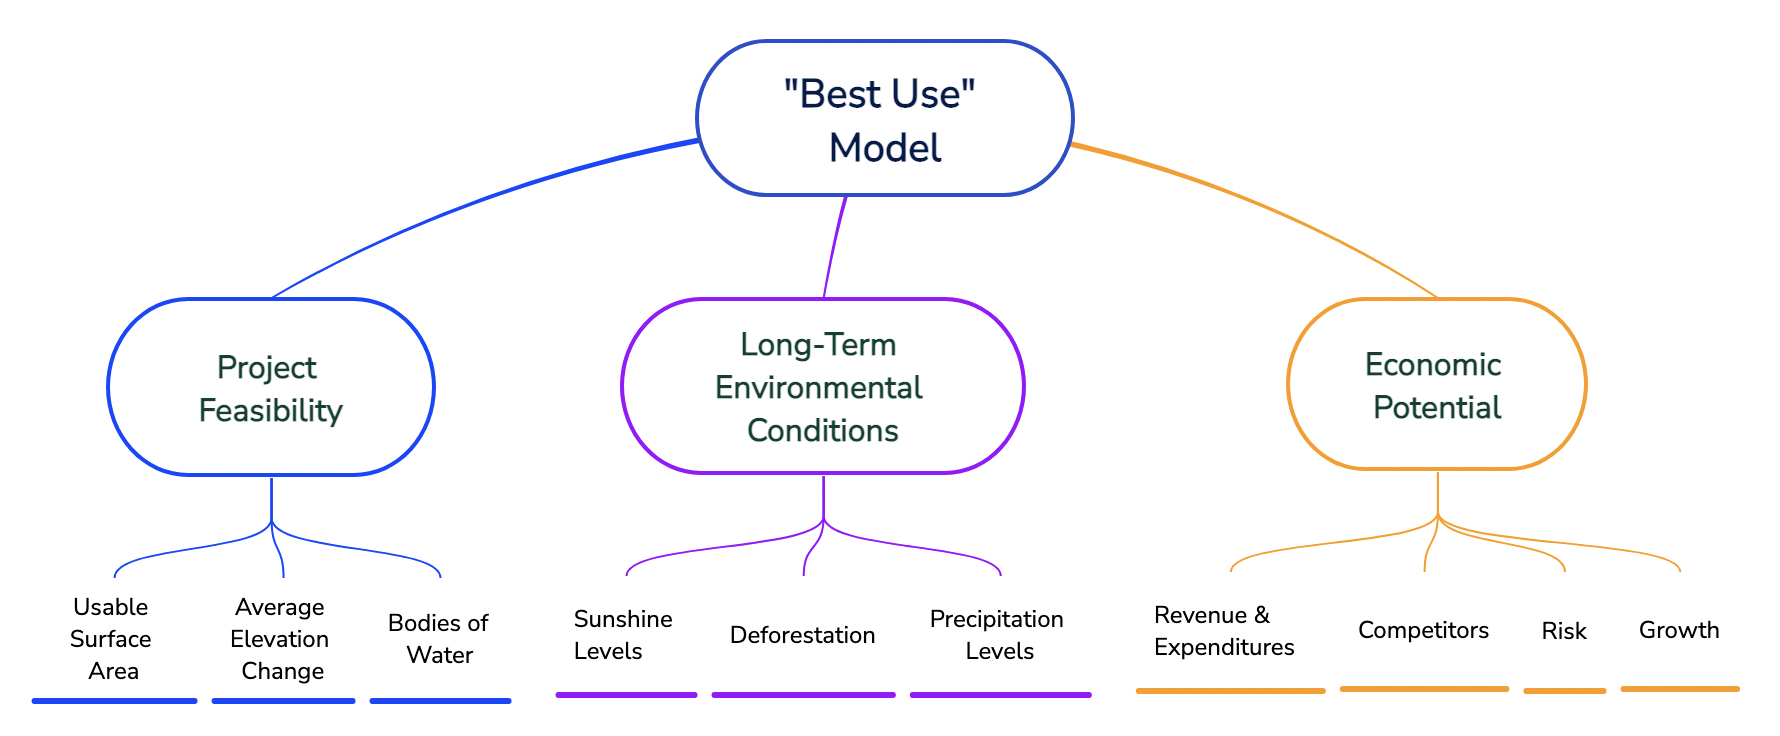
\includegraphics[scale=0.5]{figures/mindmap.png}
    \captionsetup{width=0.8\textwidth}
    \caption{\textbf{Impacting factors hierarchy tree}. A tree of all factors we considered in our decision model for choosing the "best" business. }
    \label{fig:factormindmap}
\end{figure}

\newpage
\subsection{Variables}

\begin{table}[!htbp]
\renewcommand{\arraystretch}{1.3}
%p{0.8\linewidth
    \begin{tabularx}{\textwidth}{p{0.4\textwidth} lXl}
    \toprule
    \textbf{Variable}           & \textbf{Symbol} & \textbf{Description}    \\ \midrule
    \raggedright Longitudinal Coordinate  & $x$  & Longitudinal degree at point $(x, y)$. \\
    \raggedright Latitudinal Coordinate  & $y$  & Latitudinal degree at point $(x, y)$. \\
    Region of Choice & $c_i$               &  Sliding window analysis region.  \\
    Area of Water Body & $A_{\text{water}}$               &  Area of nearest water body to region $c_i$  \\
    \raggedright Tree Coverage  & $T$  & Percentage of tree coverage at $(x, y)$. \\
    EBITDA & $EBITDA$               &  The yearly earnings of a company prior to interest, tax, depreciation, and amortization to calculate profitability \cite{adam_hayes_ebitda_nodate}.
    \\
    Earnings Per Share & $EPS$               &  The earnings per market share in the most recent yearly report of a company \cite{jason_fernando_earnings_nodate}.
    \\
    Sales Growth Percentage & $SG$               &  The percentage growth in total sales revenue over the past five years \cite{james_chen_growth_nodate}.
    \\
    Gross Profit Growth Percentage & $GPG$               &  The percentage growth in total gross profit over the past five years of a company adjusted for inflation \cite{james_chen_growth_nodate}. \\
  Standard Deviation & $\sigma$ & The standard deviation of company's market prices \cite{marshall_hargrave_standard_nodate}. \\
   Relative Strength Index & $RSI$         & A financial indicator of the validation of a stock \cite{jason_fernando_relative_nodate}.   \\
    Operating Cash Flow Ratio  & $OF$               & The availability of cash flow in a company \cite{marshall_hargrave_operating_nodate}.
    \\
    \bottomrule
    \end{tabularx}
    \end{table}

\subsection{Topographical Factors: What Makes a Project Feasible?}

One of the main concerns among land developers is the feasibility of a project. This is mainly affected by the initial state of the land, or \textit{topography}. Thus, we considered three key topographical factors: (1) Usable Surface Area, (2) Average Elevation Change, and (3) Distance to Bodies of Water. For example, flatter land may be more suited for farming, whereas mountainous land would better suit a ski resort. Likewise, distances from bodies of water may also affect land use. 

\subsubsection{Usable Surface Area}

Usable surface area is an important factor to consider because different businesses prioritize the amount of usable land differently. The usable surface area includes all land area, excluding bodies of water, as trees can be cut down to increase usable space but water cannot be removed.

In general, the surface area varies with elevation; therefore, we need to determine the elevation of specific points on the plot of land. We used ArcGIS, an online geographic information system, to discretely sample elevation data on the property, which we then used to create a continuous elevation function $E(x, y)$ where $x$ and $y$ are the longitude and latitude components, respectively \cite{esri_arcgis_nodate}. Given a point $(x, y)$ on the plot of land, the elevation function returns the altitude, or z-coordinate, in kilometers at that point. Note that we previously assumed the longitudinal and latitudinal coordinates of the Mercator Projection are rectangular.

For a region of choice $c_i$, we calculated the surface area $SA(c_i)$ using a three-dimensional surface integral to account for sloped land. The elevation data was discretely obtained, such that each $(x, y)$ coordinate is spaced $0.174$ km or $1.56 \cdot 10^{-3}$ degrees longitude and $1.04 \cdot 10^{-3}$ degrees latitude apart. Let $\frac{\partial E}{\partial x}$ be the change in elevation along the longitudinal axis and $\frac{\partial E}{\partial y}$ be the change along the latitudinal axis, where $(x, y)$ are coordinates. Then, we parameterized each surface differential as a rectangle, so that the area is the product of the lengths of the sides. Finally, we sum the \textit{usable}, or non-water, surface differential areas over the latitudinal and longitudinal axes to find the surface area of the land (Figure \ref{fig:landparcel}). 

\begin{figure}[!htbp]
\centering
    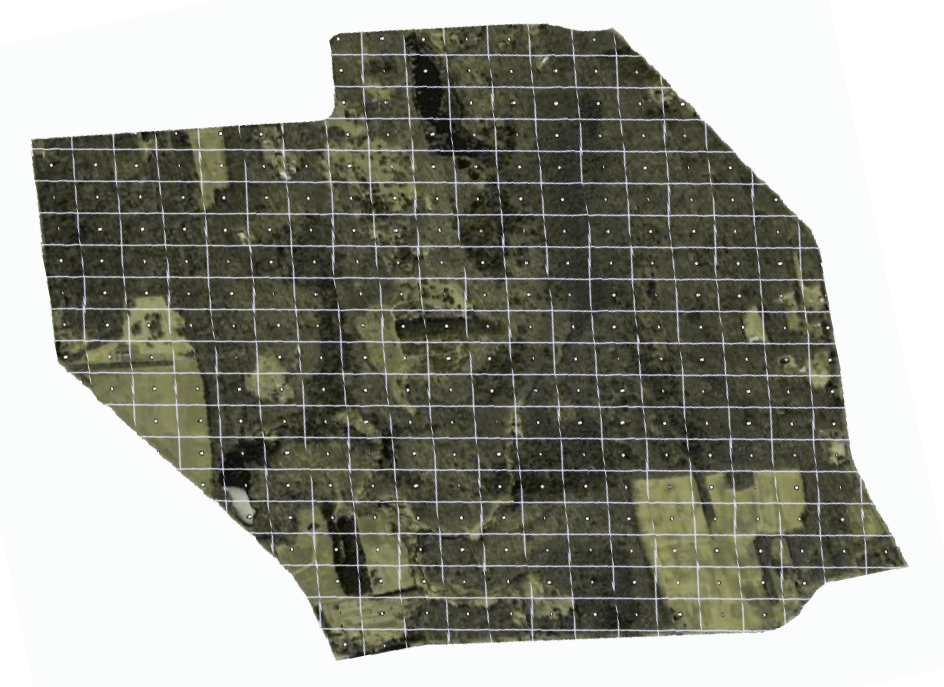
\includegraphics[scale=0.5]{figures/land_parcel_above.png}
    \captionsetup{width=0.8\textwidth}
    \caption{\textbf{A bird's eye view of the parcel of land}. Grid drawn to represent  points for our discrete $(x, y)$ coordinates.}
    \label{fig:landparcel}
\end{figure}

\begin{align}
    SA(c_i) = \sum_{i=0}^{n} \sqrt{x_i^2 + \left(\frac{\partial E}{\partial x}_i\right)^2} & \cdot \sqrt{y_i^2 + \left(\frac{\partial E}{\partial y}_i\right)^2} 
    & \forall \text{ usable }(x_i, y_i) \in c_i
    \label{Eq:SurfaceArea}
\end{align}

\subsubsection{Average Elevation Change}

Next, we created a function to determine the average elevation change given a specific area. Knowing the average change in elevation is crucial for businesses such as ski facilities, which require hills for ski trails, and for farms, which benefit from minimal elevation change. 

Similar to the surface area, in order to find average elevation change, it is necessary to use the elevation function defined previously. For elevation function $z = E(x, y)$, we find the average of the gradients along the region of choice. To calculate a gradient at point $(x, y)$, we find the magnitude of the gradient in the latitudinal and longitudinal directions. Finally, we sum and calculate the mean of all of the gradients along the region of choice $c_i$. 

\begin{figure}[!htbp]
    \centering
    % left bottom right top
    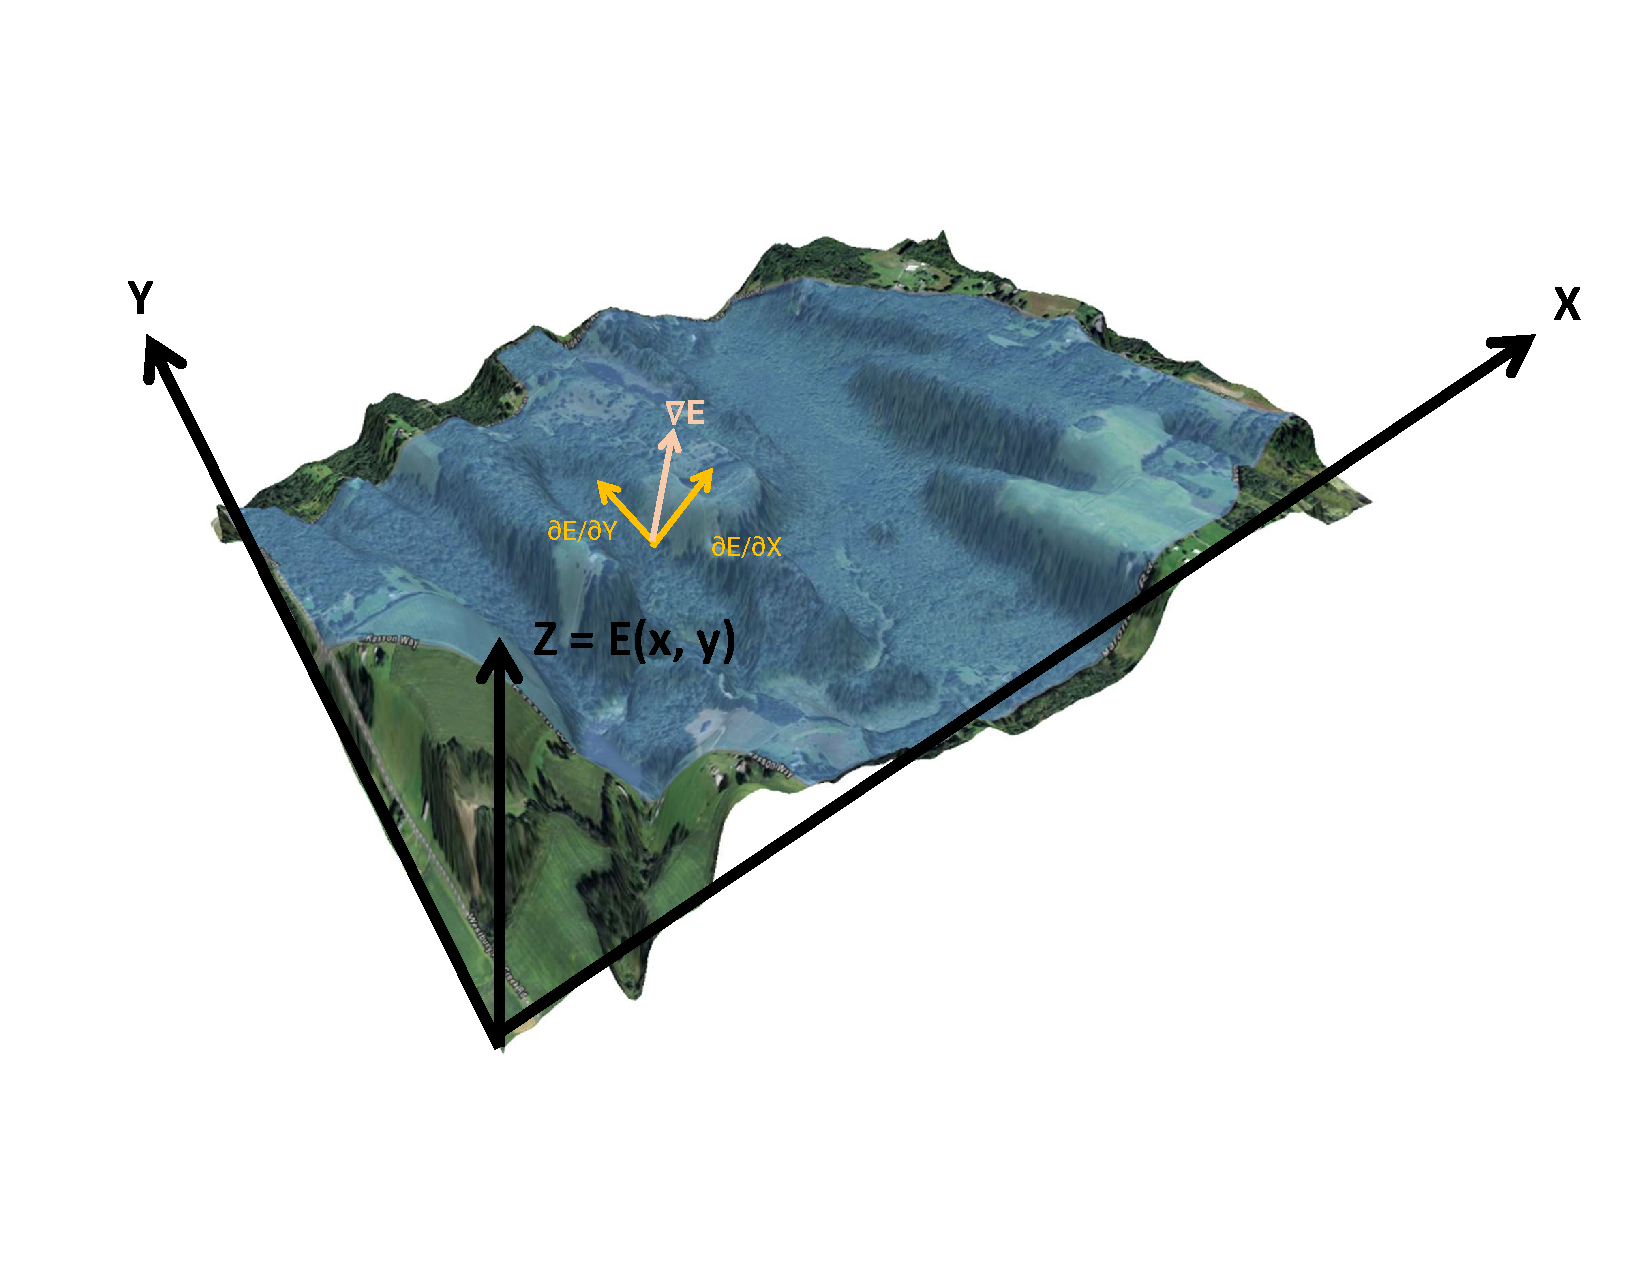
\includegraphics[trim={2cm 3.5cm 3.5cm 2cm}, scale=0.38]{figures/3dplot.pdf}
    \caption{\textbf{An isometric view of the parcel of land, representative of the plot elevation.} The visual representations for gradients by component are also shown.}
    \label{fig:isometric_parcel}
\end{figure}

%c_i represents choice and area of interest
\begin{align}
    \Bar{\Delta E}(c_i) & = \frac{1}{n} \sum_{i=0}^{n} \nabla E_i = \frac{1}{n}\sum_{i=0}^{n} \sqrt{\left(\frac{\partial E}{\partial x}_i\right)^2 + \left(\frac{\partial E}{\partial y}_i\right)^2} & \forall (x_i, y_i) \in c_i
    \label{Eq:ElevChange}
\end{align}

\subsubsection{Bodies of Water}

Next, we created a metric to quantify the impact of the nearest body of water on a given region. Proximity to bodies of water is crucial, as it can significantly impact certain businesses. For example, farms can benefit from being near a body of water to aid crop growth, while outdoor sports complexes may be less affected.


To calculate the impact of the nearest body of water on the region of choice $c_i$, we calculate this impact score function $W(c_i)$ as the root of distance in kilometers from the center of the region of choice $c_i$ and the nearest point to a river or lake as defined by the topography graphs. We chose the root function to scale the penalty for greater distances and not make their penalty disproportionate. Furthermore, define the nearest water body to have area $A_\text{water}$. Thus, we defined the impact score as follows in Equation \ref{Eq:WaterBody}.

\begin{align}
W(c_i) = \frac{A_\text{water}}{\sqrt{\sqrt{\left(\Bar{x_{c_i}} - x_{\text{water}}\right)^2 + \left(\Bar{y_{c_i}} - y_{\text{water}}\right)^2}}}
\label{Eq:WaterBody}
\end{align}

\subsection{Sustainability Factors: Long-Term Environmental Conditions}

In addition to the initial feasibility factors, we evaluated long-term environmental impacts on the land. To achieve this, we examined three climate and sustainability components that could impact business models, namely: (1) levels of sunshine, (2) levels of precipitation, and (3) the extent of deforestation.

\subsubsection{Sunshine Levels}

Sunshine levels can be a critical factor in the success of certain businesses, particularly in agriculture, where sufficient sunlight is essential for optimal crop growth. To forecast future sunshine levels in the region, we utilize a function $S(t)$, which measures sunlight in hours per month, with $t$ representing the number of months after March 2023. The total amount of sunlight over the next $n$ months can be calculated using this function as follows:

\begin{equation}
    \text{Total Sunlight} = \int_{0}^{n} S(t) dt
\end{equation}

To ensure that our model accounted for the long-term effects of global warming, such as increasing cloud cover, we aimed to move beyond a simple cyclic model of sunshine levels based on seasonal changes \cite{ceppi_observational_2021}.

We trained a Tensorflow deep learning model using over a hundred samples of sunshine data collected from Central NY, which includes several hidden layers, LSTM layers, and a prediction layer. Unlike predictive Markov models, deep learning models can handle complex patterns in data and produce more accurate predictions \cite{LSTM} \cite{martinabadi_and_tensorflow_nodate}. We utilized Long Short-Term Memory nodes in the model to process temporal data and maintain predictions throughout the model (Figure \ref{fig:lstm}).

LSTMs, as shown in Figure \ref{fig:lstm}, are often used in temporal data processing and deep learning applications. In this case, we used LSTMs to use a previous window of sunlight data to predict the next month's sunlight level. 

\begin{figure}[!htbp]
    \centering
    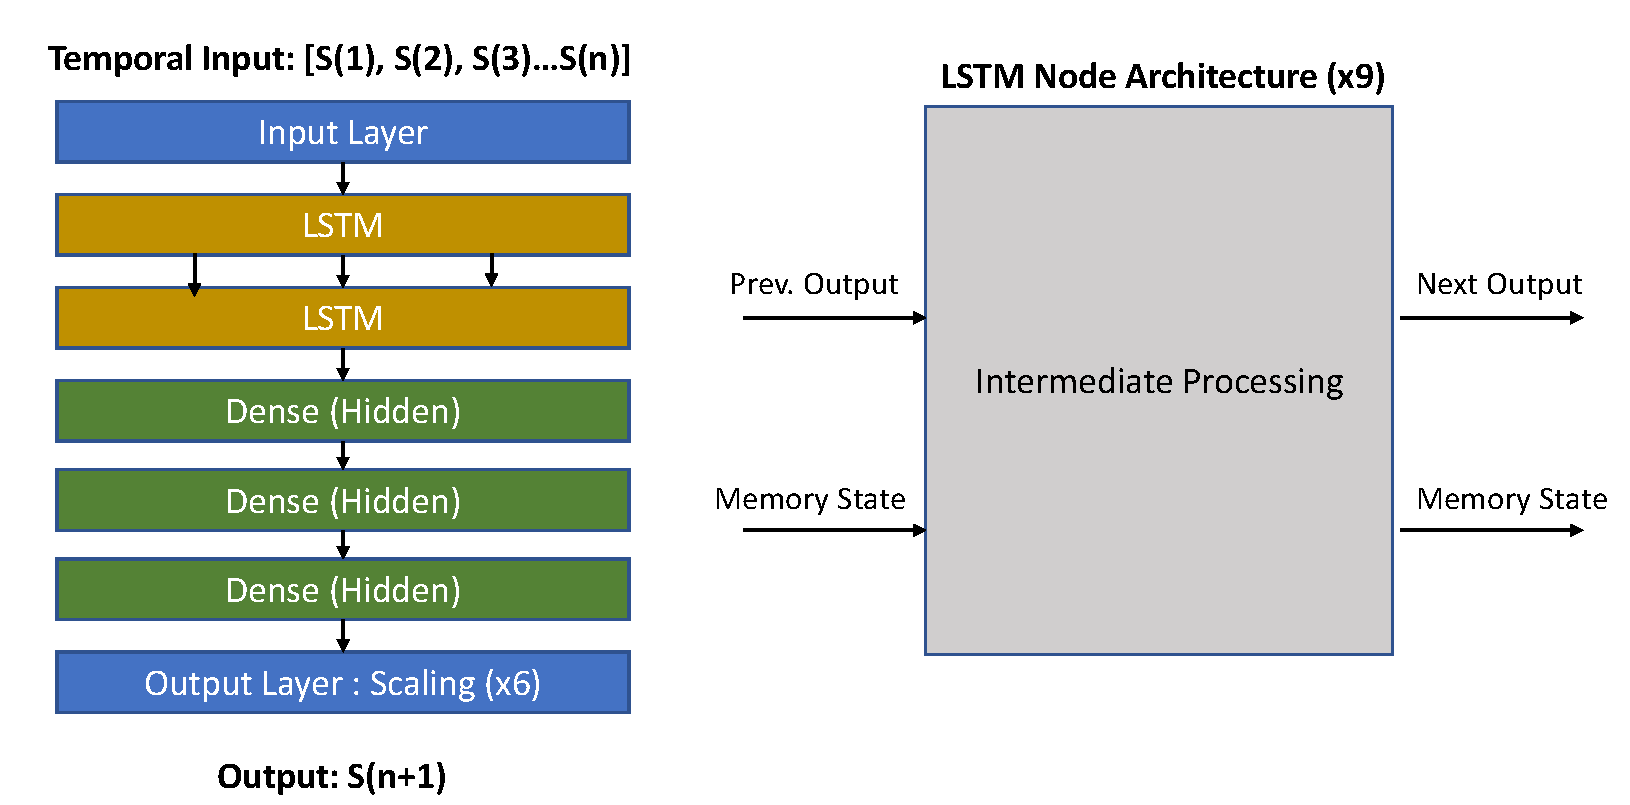
\includegraphics[scale=0.5]{figures/lstm.pdf}
    \caption{\textbf{Deep learning model architecture.} We utilized temporal-based nodes within our network to make better temporal predictions. By using a memory state, we can achieve higher accuracies \cite{LSTM}.}
    \label{fig:lstm}
\end{figure}

To optimize the prediction model's performance, we trained it on historical sunlight data for 100 iterations using the Mean Absolute Error (MAE) metric described in Equation \ref{Equation:MAE} \cite{noauthor_cnyweathercom_nodate}. The training resulted in a robust sunlight prediction model with an MAE of $15.2$. See Figure \ref{fig:sunshinepredictionfigure} for future prediction results.

\begin{equation}
    \text{MAE} = \frac{1}{n} \sum_{i=0}^{n} \left| S_{\text{true}} - S_{\text{pred}}\right|
    \label{Equation:MAE}
\end{equation}

\begin{figure}[!htbp]
    \centering
    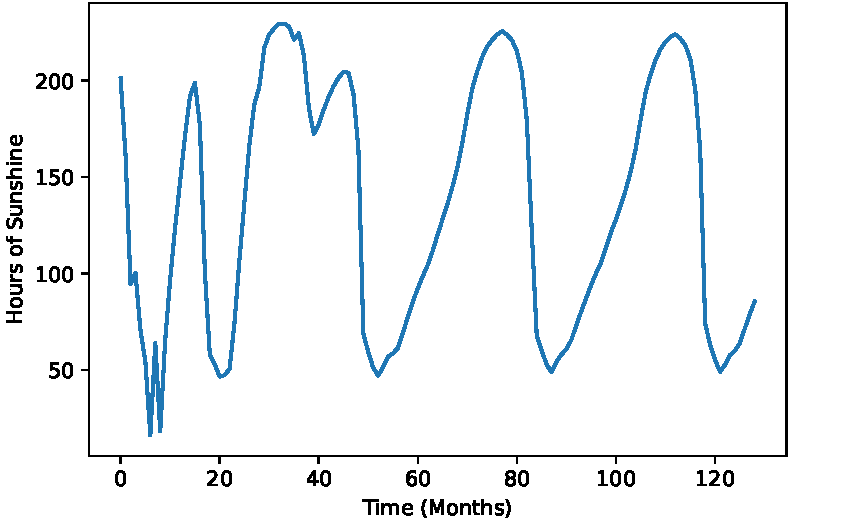
\includegraphics[scale=0.6]{figures/sunshineprediction.pdf}
    \caption{\textbf{Predicted sunshine levels.} Amount of sunshine per month after March 2023.}
    \label{fig:sunshinepredictionfigure}
\end{figure}

\subsubsection{Precipitation Levels}
Precipitation levels, like sunshine levels, can also significantly impact the success of businesses on the proposed land, depending on the objectives of individual companies.

To account for future precipitation levels and potential future outlooks for rain-dependent business models, we developed a sinusoidal regression model of best fit to represent the cyclical nature of precipitation. First, we collected historical precipitation data of monthly precipitation in inches from the past 150 years \cite{aladin_wolcott_nodate}. 

Using the window from the past 25 months, we fit a Fourier series, $R(t)$ to the data to predict future precipitation levels. We chose a Fourier series to model the cyclical data because of the varying amplitudes and periods of the data. $R(t)$ measures the monthly precipitation level in inches for month $t$ after March 2023. The typical Fourier series is in the form of Equation \ref{Equation:Fourier}. Our program to fit a Fourier series utilized a $\chi^2$ Goodness of Fit test to determine the accuracy of the calculated sinusoidal function in our model. Additionally, we set the degree of the series, $n$, to 10 to account for the variable nature of the series as well as the unique qualifications needed for a statistically relevant model. More specifically, 10 serves as the minimum degree number that can be statistically analyzed.

\begin{equation}
R(t) =a_0+\sum_{i=1}^{n}a_i + \cos(\omega x)+b_i \sin(\omega x)
\label{Equation:Fourier}
\end{equation}

Using technical computing software as shown in Appendix 4, we determined the values of the parameters of the Fourier series as shown in Table \ref{tab:fourierparams} in Appendix 1.

Using our model, we can predict the total precipitation level over the next $n$ years using Equation \ref{Eq:RainTotal}. The rain prediction chart is shown in Figure \ref{fig:RainPrediction}.

\begin{equation}
    \text{Total Rain} = \int_0^n R(t) dt
    \label{Eq:RainTotal}
\end{equation}

\begin{figure}[!htbp]
    \centering
    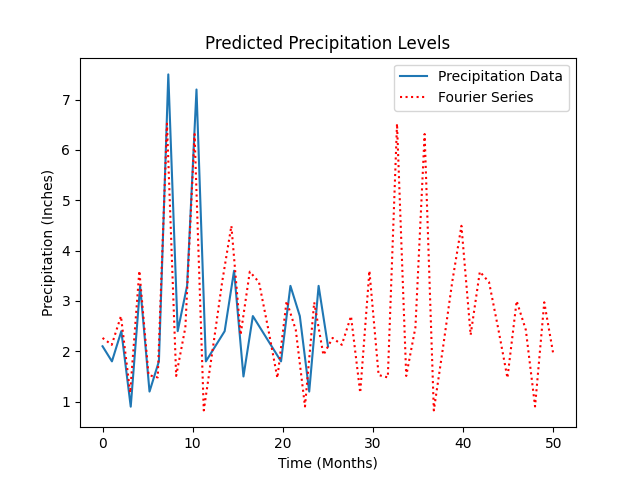
\includegraphics[scale=0.6]{figures/precipitationprediction.png}
    \caption{\textbf{Rain prediction graph over time.} The Fourier series uses the periodic attribute to project rain levels over the next several months.}
    \label{fig:RainPrediction}
\end{figure}

\subsubsection{Deforestation}
Next, we created a deforestation factor to accommodate individual business needs. For example, while some businesses prefer keeping trees, such as a ski resort for ski trails, some rely on deforestation to gain usable surface area, such as farms. Moreover, deforestation has social and cultural implications that can impact a company's revenue, as seen with agritourism centers that rely on community tourism. 

To consider the impact of deforestation on community views, we define a function $D(c_i)$ for the region of interest $c_i$, which measures the number of trees and natural foliage removed while starting a business. We assume that as the number of removed trees increases, the business's impact on community views also increases. The tree cover percentage at a specific coordinate $(x, y)$ is denoted as $T(x, y)$.

% we assume everything is deforested

We express the deforestation function as Equation \ref{Eq:deforestation}, which integrates the percentage forest coverage over the region of interest to determine the total forest coverage removed in $\text{km}^2$.

\begin{align}
    D(c_i) & = \iint_{c_i} T(x, y) dx dy & \forall (x, y) \in c_i
    \label{Eq:deforestation}
\end{align}

\subsection{Economic Factors: Time to Make Money}
Lastly, we determined that economic factors, such as potential revenue, growth, expenditures, risk, and nearby competitors, will affect how well a business will "fit" in the plot of land.

In order to fully account for these factors we conducted a thorough market analysis for each business option. In our analysis, we determined the two most \textit{similar} publicly-held companies for each business option, denoted as $sb_k$. We determined similarity between businesses and business choice $b_i$ by company location and, most importantly, company mission. From each similar company, we collected yearly financial statements, stock prices, and financial indicators to determine company health.

In each of the sub-factors below, we normalized the output values to be near 0 to 1. The normalization was performed to allow addition of the scores without heavy skew caused by large discrepancies or outliers.

\subsubsection{Revenue and Expenditures}

We predict business model $b_i$'s potential revenue and expenditures, and consequentially, profit. In Equation \ref{Eq:profitscore}, we developed a profit score $P(b_i)$ of business choice $b_i$ as a function of \textit{similar} business profit performances. First, we calculated $EBITDA$ margins of the $n$ \textit{similar} businesses for business choice $b_i$, which are an evaluation of earnings per total revenue. The formula for $EBITDA$ margin can be found in Equation \ref{Eq:EBITDA}, which indicates the potential profitability of \textit{similar} businesses. Next, we calculated Price to Earnings $PE$ ratios per $n$ \textit{similar} businesses to factor in the value of the company. These financial indices are collected from the most recent yearly report. The formula for the $PE$ ratio can be found in Equation \ref{Eq:PERatio}.

\begin{equation}
     \text{ EBITDA Margin} = \frac{\text{Earnings Before Interest, Tax, Depreciation, Amortization}}{\text{Total Revenue}}
    \label{Eq:EBITDA}
\end{equation}

\begin{equation}
    PE \text{ Ratio} = \frac{\text{Market Value Per Share}}{EPS}
    \label{Eq:PERatio}
\end{equation}

Since a higher $EBITDA$ margin and lower $PE$ ratio (near 10) is desirable for a profitable and high-earning company, we developed the following weighted average function for profit score $P(b_i)$ in Equation \ref{Eq:profitscore}. Since $EBITDA$ margin is a percentage between 0-1, we were able to make sure that the score was normalized. Furthermore, an optimal $PE$ ratio would be near 5 to 10 since a lower $PE$ ratio is better, so we divided 10 by the $PE$ ratio to create a normalized score. 

\begin{equation}
    P(b_i) = \frac{1}{n} \sum_{k=0}^n  EBITDA \text{ Margin}_{sb_k} + \frac{10}{PE \text{ Ratio}}_{sb_k}
    \label{Eq:profitscore}
\end{equation}

\subsubsection{Growth}
Next, we developed a growth score $G(b_i)$ to assess the potential growth in a company. This was used to further evaluate the long-term goals of a business model $b_i$. First, we considered \textit{similar} company sales and inflation-adjusted gross profit growth over the past five years as percentages. Next, we denote sales growth as $SG_{sb_k}$ and gross profit growth as $GPG_{sb_k}$, both of which are expressed as percentages. Then, we normalized these percentage scores by dividing them by one hundred and setting their weights as $0.3$ and $0.7$ to scale the scores between 0 and 1. These growth percentages were included to measure potential growth in our business choice. 

We defined our growth score to be Equation \ref{Eq:growthscore} as a weighted average of sales growth and gross profit growth over all $n$ \textit{similar} businesses $sb_k$. Thus, the higher the growth score, the greater potential growth this company has. Since we decided that profitability depends on gross profit growth more than sales growth, our weighted average leaned towards $GPG$. 

\begin{equation}
    G(b_i) = \frac{1}{n} \sum_{k=0}^n \frac{1}{100} \left( 0.3 SG_{sb_k} + 0.7 GPG_{sb_k} \right)
    \label{Eq:growthscore}
\end{equation}

\subsubsection{Risk}
We define the \textit{risk} function as the score $\zeta(b_i)$ of company failure. The greater the $\zeta$ score, the greater the probability of company bankruptcy or failure and the lower the $\zeta$ score, the lower the probability of company failure. 

To analyze the \textit{risk} of a potential company $b_i$, we find a weighted average of current risk-indicators such as the Standard Deviation of Market Prices $\sigma$, Relative Strength Index $RSI$, and Operating Cash Flow Ratio $OF$ financial indicators in \textit{similar} businesses, $sb_k$. Standard deviation, or $\sigma$, is an indicator of volatility, or instability, of a company. Furthermore, indicators such as $RSI$ and $OF$ are measures of risk and stability, respectively. More specifically, these financial indices are collected from the most recent yearly report. We define risk score as a weighted mean over the $n$ \textit{similar} businesses of the risk indicators in Equation \ref{Eq:Risk}. 

\begin{equation}
    \zeta(b_i) = \sum_{k=0}^{n} \frac{1}{100} \sigma_{sb_k} + \frac{1}{80} RSI_{sb_k} - \frac{1.1}{OF_{sb_k}}
    \label{Eq:Risk}
\end{equation}

Furthermore, we scaled the $RSI$ index by 80 since greater RSI indicates overvalued companies, and thus a greater risk. Lastly, we divided 1.1 by the $OF$ ratio and subtracted this factor. Ratios greater than 1.1 would signify a decreased risk, since a greater cash flow suggests stability in a company. A lower or negative $OF$ would signify greater risk, thus we used the reciprocal of $OF$. 

\subsubsection{Competitors}
If a potential business model has nearby competitors within a radius of 25 miles, it will negatively impact the potential business model $b_i$. The farther the competing business is, the less of an impact the competitor will have. Thus, we define our competitor function (within 25 miles) $\Upsilon(b_i)$ of business model $b_i$ as the sum of the root of the distance in kilometers between the 3 $\text{km}^2$ plot of land and the $n$ competitor(s) as seen in Equation \ref{Eq:competitorscore}. 

\begin{equation}
    \Upsilon(b_i) = \sum_{k=0}^n \frac{1}{\sqrt{\text{distance}_{k}}}
    \label{Eq:competitorscore}
\end{equation}

This score is normalized as the distances are in the denominator, thus the individual score per competitor will be near or less than 1. 

\subsubsection{Combined Economic Score}
Since each score is normalized, we can add the scores to achieve a total economic score $E_c$ (Equation \ref{Eq:combinedeconomicscore}). We subtracted negatively-affecting scores such as risk and competitors and added the positively-affecting scores such as profitability and growth.

\begin{equation}
    E_c(b_i) = P(b_i) + G(b_i) - \zeta(b_i) - \Upsilon(b_i)
    \label{Eq:combinedeconomicscore}
\end{equation}

\subsubsection{Collected Financial Data}
For input values to the financial model scores, all collected data was obtained from publicly held companies who maintained companies and sites similar to our land plot. The full table of values can be found in Table \ref{tab:financialdata} \cite{noauthor_vail_nodate, noauthor_adecoagro_nodate, noauthor_jbs_nodate, noauthor_grupo_nodate, noauthor_first_nodate, noauthor_cubicfarm_nodate, noauthor_carnival_nodate, noauthor_american_nodate, noauthor_farmland_nodate, noauthor_hormel_nodate, noauthor_maxeon_nodate, noauthor_hydrofarm_nodate, noauthor_general_nodate, noauthor_academy_nodate}.

\subsection{Calculating a "Best" Score}
In order to account for the three major areas in our decision-making for planning the use of the land, we designed a decision matrix. The proposed decision matrix calculates each topographical, sustainability, and economic factor for each region of choice and business model. Then, we scale using a normal distribution to the resulting values of each factor to find out which factors are stronger in each region of interest. Lastly, we choose the business model with rankings of factors that best align with the region of interest. 

\subsubsection{Combined Scores Matrix}
For each region of interest $c_i$ and business model $b_i$, a \textit{raw} combined score matrix $\textbf{RS}$ will be calculated as a vector of values from each individual factor. 

\begin{equation*}
    \textbf{RS} = \begin{bNiceMatrix}[first-row,first-col]
    & SA & \Delta E & W & S & R & D & Ec \\
    \text{Sports Complex } (b_1) & SA(c_i) & \Delta E(c_i) & W(c_i) & \int\limits_0^n S(t)dt &  \int\limits_0^n R(t)dt & D(c_i) &  E_c(b_i) \\
    \text {Ski Facility } (b_2) & \cdots &  &  & &  &  &  \\
    \text{Crop Farm } (b_3) &  &  \cdots &  &  &  &  &  \\
    \text{Grazing Farm } (b_4) &  &  & \cdots &  &  &  &  \\
    \text{Regen. Farm } (b_5) &  &  &  & \cdots &  &  &  \\
    \text{Solar Array } (b_6) &  &  &  &  & \cdots &  &  \\
    \text{Agrivoltaic Farm } (b_7) &  &  &  &  &  & \cdots &  \\
    \text{Agritourist Center } (b_8) &  &  &  &  &  &  & \cdots  \\
    \end{bNiceMatrix}
\end{equation*}

\subsubsection{High-Low Matrix}
The criteria considered in this matrix were categorized into three major groups: Topography, Sustainability, and Economic Factors. We defined the \textit{High-Low Matrix} based on the priorities of each business model for the feasibility factors. For each value $HL_{ij}$ in \textit{High-Low Matrix} \textbf{HL}, we assign a 1, 0, or -1. We assign a 1 to $HL_{ij}$ if business choice in row $i$ desires a high output in the score of column $j$. Consequentially, we assign a -1 to $HL_{ij}$ if business choice in row $i$ desires a low output in the score of column $j$. Lastly, we assign a 0 if the business desires a middle-ground output in the score column or if there is no relevance of the score to the business.

\begin{equation}
    \textbf{HL} = \begin{bNiceMatrix}[first-row,first-col]
    & SA & \Delta E & W & S & R & D & Ec \\
    \text{Outdoor Sports Complex} & 1 & -1 & 0 & 1 & 0 & 0 & 1 \\
    \text {Ski Facility} & 1 & 1 & 1 & 0 & -1 & -1 & 1 \\
    \text{Crop Farm} & 1 & -1 & 1 & 1 & 1 & 1 & 1 \\
    \text{Grazing Farm} & 1 & 0 & 1 & 1 & 1 & 1 & 1 \\
    \text{Regenerative Farm} & 1 & 0 & 0 & 1 & 1 & -1 & 1 \\
    \text{Solar Array} & 1 & 0 & 0 & 1 & 0 & 1 & 1 \\
    \text{Agrivoltaic Farm} & 1 & -1 & 1 & 1 & 1 & 1 & 1 \\
    \text{Agritourist Center} & 1 & -1 & 1 & 1 & 0 & -1 & 1 \\
    \end{bNiceMatrix}
\end{equation}

The factors for \textbf{topography} are as listed and each \textit{High-Low} value is discussed below. 
\begin{enumerate}
    \item Usable Surface Area $(SA) $
        \begin{quote}
            In this case, all businesses want to utilize as much space as they can; therefore, all companies want a high usable surface area or a score of 1.
        \end{quote}
    \item Elevation Change $(\Delta E)$
        \begin{quote}
            Ski facilities benefit from significant elevation changes for ski trails, while outdoor sports complexes and crop farms benefit from less elevation change or flat land. Grazing farms, regenerative farms, and solar arrays are indifferent to elevation change.  
        \end{quote}
    \item Water (W)
        \begin{quote}   
            The two primary businesses that benefit from being near a body of water are agricultural farms and ski facilities; proximity to water increases irrigation quality, and water can be used to create fake snow. Other listed businesses do not require close proximity to a body of water, thus receiving lower values in the matrix. 
        \end{quote}
\end{enumerate}

The factors for \textbf{sustainability} are as listed and each \textit{High-Low} value is discussed below.
\begin{enumerate}
    \item Sunshine Amounts $(S)$
        \begin{quote}
            In most cases, high sunshine levels are beneficial for crop growing, harvesting energy from solar panels, or attracting tourists with good weather. The only company that would not need sunshine is a ski facility since it is possible to ski when it is lightly snowing as well as later in the evening once the sun has set.
        \end{quote}
    \item Rain Levels $(R)$
        \begin{quote}
            All farms benefit from rain to aid crop growth. However, a solar array farm and an agritourist center are indifferent to rain since the former does not include any crop growing. The latter requires a balance between rain for crops and good weather to attract tourists. Conversely, a ski facility would not benefit from rain since it could cause snow on its trails to melt. 
        \end{quote}
    \item Deforestation Levels $(D)$
        \begin{quote}
             For most farms, deforestation is necessary for additional crop growth as it increases usable surface area. Regenerative farms and agritourist centers are exceptions, as they prioritize sustainability and community views. Ski facilities also do not benefit from deforestation, as trees are beneficial to ski trails. Outdoor sports complexes are generally indifferent to deforestation since their land is not heavily forested, but they may cut down trees if needed.
        \end{quote}
\end{enumerate}

Lastly, since all business models $b_i$ would desire a greater economic score, we set the \textit{High-Low} value to be 1 for all companies. 

\subsubsection{Importance Matrix}

We created an importance matrix to assess the significance of different factors for each company, taking into account their unique values and objectives. For instance, sunshine is crucial for solar arrays to generate energy, making it the top priority. In contrast, elevation and economy are more essential for ski facilities. We conducted this evaluation for all eight types of businesses in our model, and the resulting importance matrix can be found in Figure \ref{fig:importancematrix}.

More specifically, we ranked each factor for each business on a scale of 1 to 7, 1 being most important for that company and 7 being least important. We did this by considering the values of each company and what would be most important for the success of each business. Detailed derivations of each rank for each company are discussed in Appendix 7.

We decided that an importance matrix would be the most suitable approach for our model and would minimize bias when scaling each factor for each company. Unlike a weighted scale of importance, a ranking system considers the varying significance of different factors to different businesses.

\begin{figure}[!htbp]
\centering
    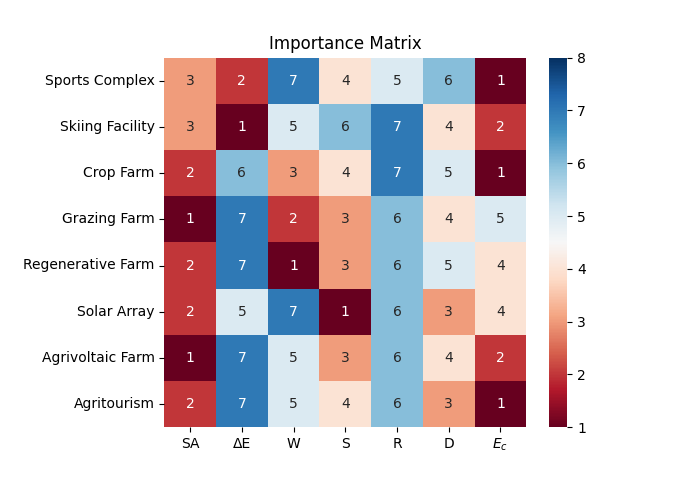
\includegraphics[scale=0.6]{figures/correlationmatrix.png}
    \captionsetup{width=0.9\textwidth}
    \caption{\textbf{Importance Matrix}. Approximated rankings of importance for matrix \textbf{I} for each business model $b_i$. }
    \label{fig:importancematrix}
\end{figure}

\subsubsection{Final Score Calculation}
Because the Raw Score calculation is challenging to compare and analyze, we devised a new method for calculating the final score. Our approach employs a normal distribution, z-scores, and rank correlation analysis techniques. Figure \ref{fig:finalscorecalc} visually depicts our final score calculation.

First and foremost, we normalized the raw scores from matrix $\textbf{RS}$ by column, such that value $RS_{ij}$ would be normalized by the values of column $j$ and corresponding column $j$'s in other raw score matrices from the sliding window analysis in Part 2. We conducted normalization in order to analyze factors with respect to mean values, so we normalized the raw score using the z-score of $RS_{ij}$. 

Thus, for raw score matrix $\textbf{RS}$, we are to obtain a new matrix $\textbf{RS'}$ of z-scores for each score $RS_{ij}$. However, since some scores are more desirable as negative or lower values while others are more desirable as higher values, we utilized the \textit{High-Low Matrix} to account for these stark differences. For each row $i$ in z-score matrix $\textbf{RS'}$, we perform element-wise multiplication to row $i$ of matrix $\textbf{HL}$. Thus, we are able to obtain appropriately scaled values with respect to desirable outcomes. 

Lastly, our model considers rank correlation in order to find the business model best fit for our final scores. In order to compare our z-scores from matrix $\textbf{HL'}$, we used the Spearman's Rank Correlation Coefficient ($\rho$) to find a business model that best fits the rankings from the Importance Matrix \textbf{I} (Figure \ref{fig:importancematrix}). We rank the z-scores from matrix $\textbf{RS'}$ to compare to matrix $\textbf{I}$. The Spearman's Rank Correlation Coefficient finds the correlation from a scale of -1 to 1, with 1 representing the highest correlation in rankings, and thus the best business model choice has the greatest coefficient \cite{noauthor_182_nodate}. The formula for the Spearman's Rank Correlation Coefficient ($\rho$) is described in Equation \ref{Eq:spearmancoeff} where $d_i$ is the difference in rankings between the $i$th pair of rankings and $n$ is the total number of rankings.

\begin{equation}
    \rho = 1 - \frac{6\sum d_i^2}{n(n^2-1)}
    \label{Eq:spearmancoeff}
\end{equation}

Therefore, the business model $b_i$ that has the \textbf{greatest Spearman Correlation Coefficient is the optimal choice}.

\begin{figure}[!htbp]
    \centering
    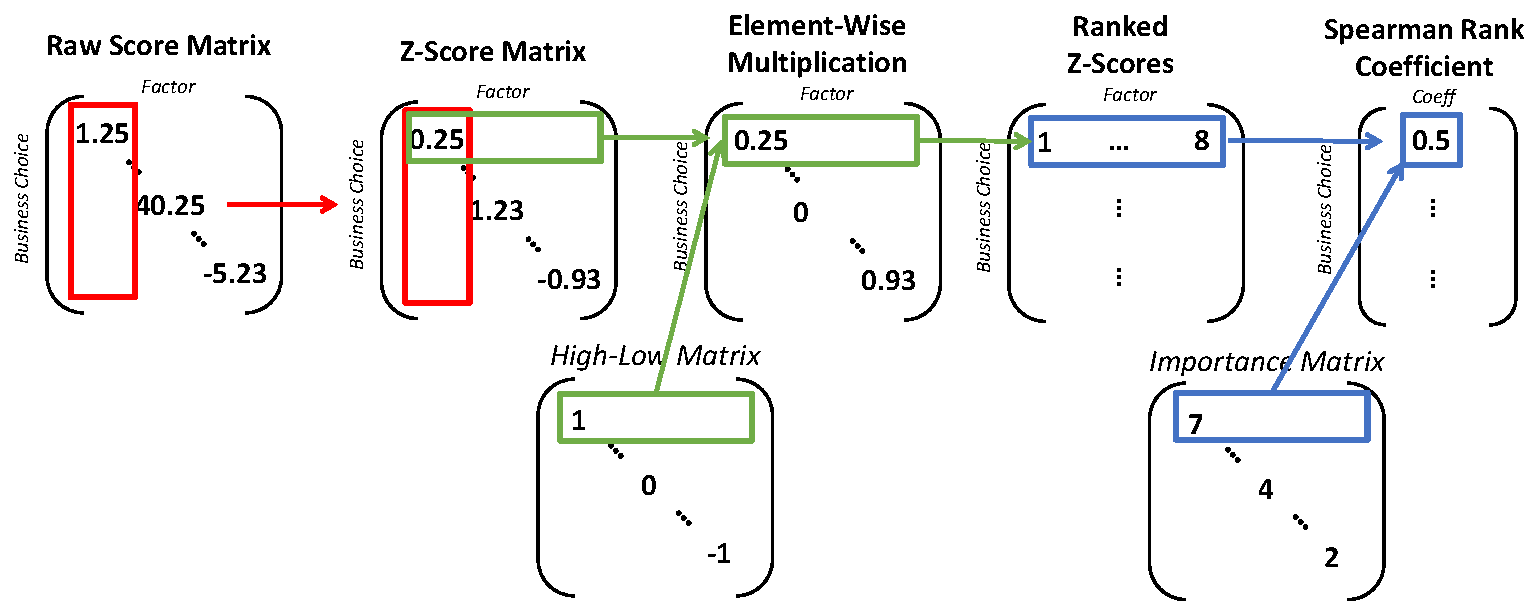
\includegraphics[scale=0.55]{figures/matrixvisual.pdf}
    \caption{\textbf{Flowchart for final score calculation.} Utilizes z-scores, the \textit{High-Low Matrix}, and Rank Correlation analysis techniques.}
    \label{fig:finalscorecalc}
\end{figure}

\section{Part 2: Applying Our Model to Specific Scenarios}
\subsection{Sliding Window Analysis}
We utilized a sliding window analysis technique to assess our decision model on the plot of land. This approach involved applying the decision model to various windows throughout the land. Using a sliding window, we could determine the best business model for each section of the land.

As shown in Figure \ref{fig:slidingwindow}, we partitioned the plot of land with two, one, one, and no partition. From each partition, we applied our decision model onto the window to calculate the raw score, z-scores, and conduct rank correlation analysis. The implementation for our sliding window analysis can be found in Algorithm \ref{alg:slidingwindows}. In order to collect data on the topographic variables; surface area, elevation change, and distance from water, we decided to work with ArcGIS.  

Additionally, once each window is analyzed separately using our model, we compared all the windows using our previously discussed decision method in order to finalize which business choice best fits each window.

\begin{figure}[!htbp]
    \centering
    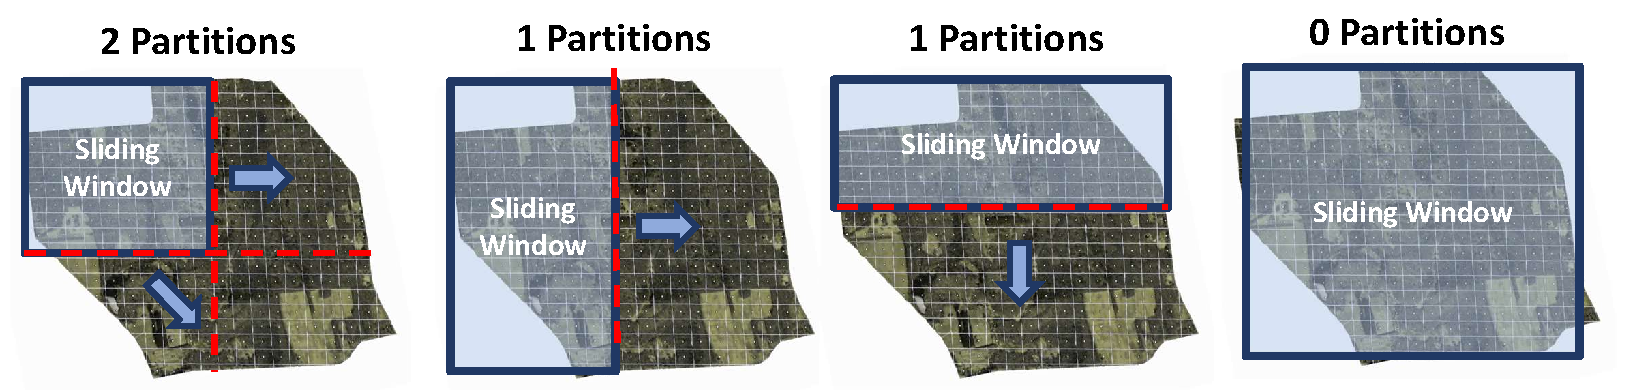
\includegraphics[scale=0.58]{figures/slidingwindow.pdf}
    \caption{\textbf{Sliding window visualization.} Displays four sliding window considerations with 2, 1, 1, and 0 partitions, respectively.}
    \label{fig:slidingwindow}
\end{figure}

\begin{algorithm}[!htbp]
\caption{\textbf{An algorithm to implement sliding windows.} X is the score matrix, HL is the \textit{High-Low Matrix}, I is the importance matrix, and Y is the vector of the final Spearman's Coefficients.}
\label{alg:slidingwindows}

$X \gets [[0...0]...[0...0]]$\;
$HL \gets [[1..0..-1]...[0..-1..1]]$\;
$I \gets [1..3..8]...[5..2..7]]$\;
$Y \gets [0...0]$\;
\For{$W \in \text{WINDOWS}$} {
    \For{$B \in \text{BUSINESSES}$} {
        \For{$row \in [0, 9]$} {
        
            $X[row, :] \gets \text{RAW SCORE}_{W, B}^T$\;
            $X[row, :] \gets \text{Z-Score}(X[row, :])$\;
            $X[row, :] \gets X[row, :] * HL[row, :]$\;
            $Y[row] \gets \text{SPEARMAN}(I[row, :], X[row, :])$];
            
        }
    }
}

% https://texdoc.org/serve/algorithm2e/0
\end{algorithm}

\subsection{Results}

\subsubsection{Two Partitions}

When the plot of land is partitioned twice into four regions, we calculated the final Spearman's Coefficients for each region of choice $c_i$. The results from the previously discussed decision model can be found in Table \ref{tab:spearman2x2}. Thus, the optimal business choice for each region is the business $b_i$ with the highest Spearman's Coefficient. The optimal business choice for dividing the region into 4 parts is a \textbf{grazing farm, agrivoltaic farm, and sports complex} in the formation of Figure \ref{fig:businessallocation2x2}.

\begin{table}[!htbp]
    \begin{tabularx}{\textwidth}{XlXlXlXl}
        \toprule
        & \multicolumn{4}{c}{\textbf{Spearman Rank Correlation Coefficient}} 
        \\
        \textbf{Business Model} & \textbf{Top Left} & \textbf{Top Right} & \textbf{Bottom Left} & \textbf{Bottom Right}\\
        \midrule
        Sports Complex & $0.161$ & $0.125$ & $-0.054$ & $\textbf{0.482}$ \\
        Skiing Facility & $-0.143$ & $-0.321$ & $-0.179$ & $-0.036$ \\
        Crop Farm & $-0.250$ & $-0.357$ & $-0.036$ & $-0.214$ \\
        Grazing Farm & $\textbf{0.286}$ & $\textbf{0.679}$ & $0.000$ & $0.393$ \\
        Regen. Farm & $-0.518$ & $-0.339$ & $-0.268$ & $-0.089$ \\
        Solar Array & $-1.268$ & $-0.839$ & $-0.696$ & $-0.268$ \\
        Agrivoltaic Farm & $-0.786$ & $-0.643$ & $\textbf{0.071}$ & $-0.214$ \\
        Agritourist Center & $-0.571$ & $-0.643$ & $0.070$ & $-0.250$ \\
        \bottomrule
    \end{tabularx}
    \caption{\textbf{Final Spearman's Coefficients for 2x2 partitioned land.} Raw scores and intermediate scores can be found in Appendix 8.}
    \label{tab:spearman2x2}
\end{table}

\begin{figure}[!htbp]
    \centering
    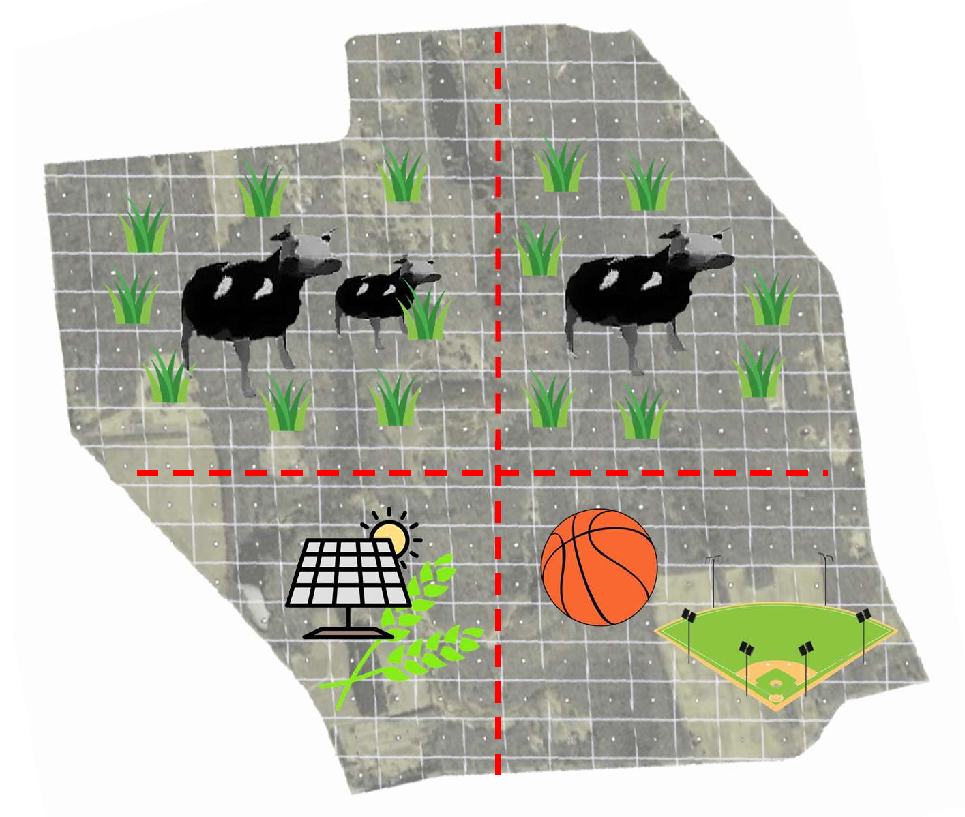
\includegraphics[scale=0.3]{figures/2x2businesschoice.pdf}
    \caption{\textbf{Visual representation of optimal business choices.}}
    \label{fig:businessallocation2x2}
\end{figure}

\subsubsection{A Singular Vertical Partition}
After dividing the plot of land into two vertical regions, we calculated the final Spearman's coefficients for each region of choice $c_i$. Table \ref{tab:spearman1vert} displays the decision model results, which reveal that the \textbf{best business choice for the left region would be an agrivoltaic farm and for the right region would be an outdoor sports complex}. See Figure \ref{fig:businessallocation1vert} for the corresponding business allocation visualization.

\newcolumntype{b}{X}
\newcolumntype{s}{>{\hsize=.5\hsize}X}
\begin{table}[!htbp]
    \begin{tabularx}{\textwidth}{bss}
        \toprule
        & \multicolumn{2}{c}{\textbf{Spearman's Rank Correlation Coefficient}} 
        \\
        \textbf{Business Model} & \textbf{Left} & \textbf{Right}\\
        \midrule
        Sports Complex & $-0.054$ & $\textbf{0.554}$ \\
        Skiing Facility & $-0.179$ & $-0.036$  \\
        Crop Farm & $-0.036$ & $-0.286$  \\
        Grazing Farm & $-0.179$ & $0.464$ \\
        Regen. Farm & $-0.268$ & $-0.161$ \\
        Solar Array & $-0.696$ & $-0.304$  \\
        Agrivoltaic Farm & $\textbf{0.071}$ & $-0.536$  \\
        Agritourist Center & $0.070$ & $-0.5$  \\
        \bottomrule
    \end{tabularx}
    \caption{\textbf{Final Spearman's Coefficients for vertically partitioned land.} Raw scores and intermediate scores can be found in Appendix 8.}
    \label{tab:spearman1vert}
\end{table}

\begin{figure}[!htbp]
    \centering
    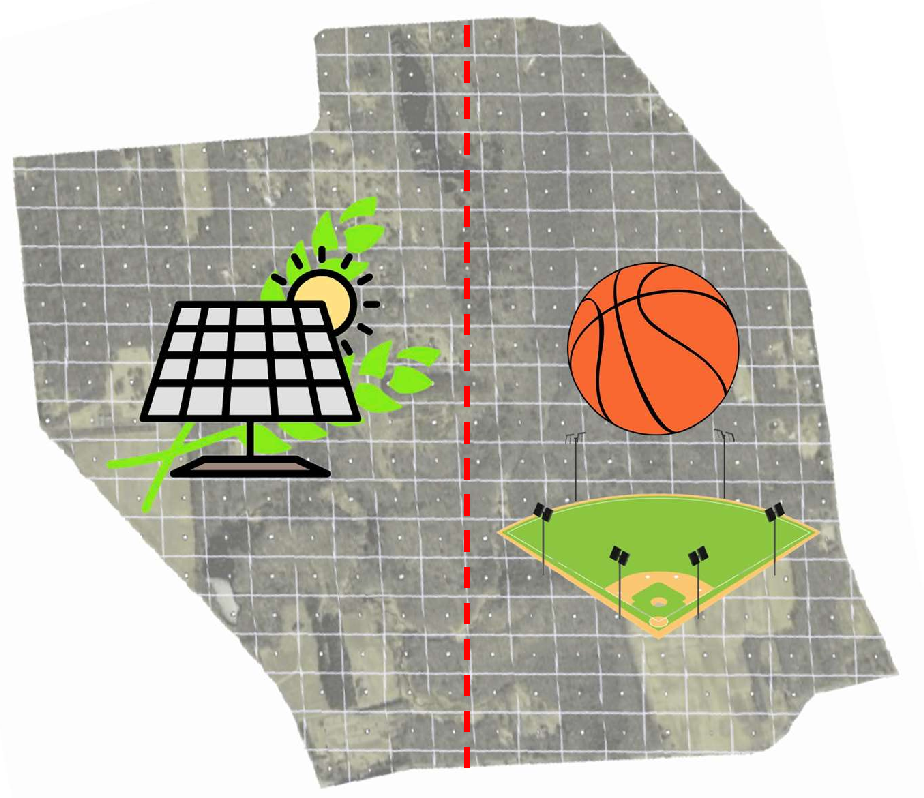
\includegraphics[scale=0.3]{figures/spearman1vert.pdf}
    \caption{\textbf{Visual representation of optimal business choices.}}
    \label{fig:businessallocation1vert}
\end{figure}

\subsubsection{A Singular Horizontal Partition}
When the plot of land is partitioned into two horizontal regions, we calculated the final Spearman's Coefficients for each region of choice $c_i$. The results from the previously discussed decision model can be found in Table \ref{tab:spearman1horiz}. Thus, the optimal businesses for this partitioning would be a \textbf{grazing farm and a cross-country skiing facility}, as shown in Figure \ref{fig:businessallocation1horiz}.

\begin{table}[!htbp]
    \begin{tabularx}{\textwidth}{bss}
        \toprule
        & \multicolumn{2}{c}{\textbf{Spearman's Rank Correlation Coefficient}}
        \\
        \textbf{Business Model} & \textbf{Top} & \textbf{Bottom}\\
        \midrule
        Sports Complex & $0.125$ & $0.018$ \\
        Skiing Facility & $-0.214$ & $\textbf{0.107}$  \\
        Crop Farm & $-0.357$ & $-0.107$  \\
        Grazing Farm & $\textbf{0.321}$ & $0.106$ \\
        Regen. Farm & $-0.446$ & $-0.268$ \\
        Solar Array & $-0.839$ & $-0.696$  \\
        Agrivoltaic Farm & $-0.786$ & $-0.321$  \\
        Agritourist Center & $-0.679$ & $-0.000$  \\
        \bottomrule
    \end{tabularx}
    \caption{\textbf{Final Spearman's Coefficients for horizontally partitioned land.} Raw scores and intermediate scores can be found in Appendix 8.}
    \label{tab:spearman1horiz}
\end{table}

\begin{figure}[!htbp]
    \centering
    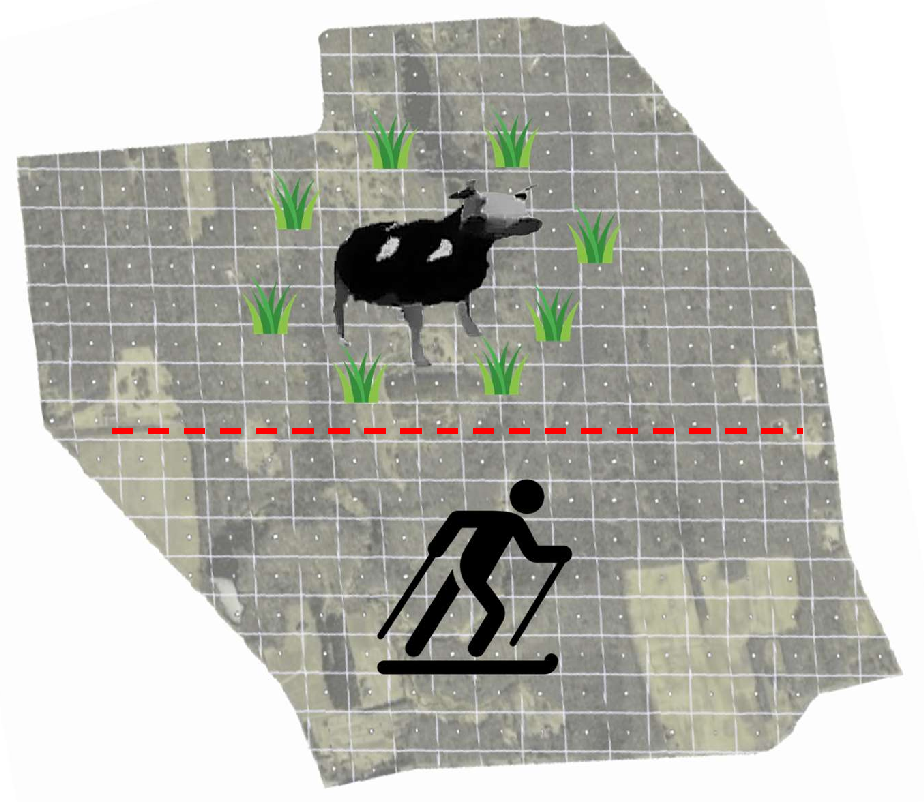
\includegraphics[scale=0.3]{figures/businesschoice1horiz.pdf}
    \caption{\textbf{Visual representation of optimal business choices.}}
    \label{fig:businessallocation1horiz}
\end{figure}

\subsubsection{Zero Partitions}
When the plot of land is not partitioned and the window contains the entire region, we calculated the final Spearman's Coefficients for the entire region. The results from the previously discussed decision model can be found in Table \ref{tab:spearman0}. Thus, the optimal business choice if the land was not divided would be a \textbf{grazing farm}.

\begin{table}[!htbp]
    \begin{tabularx}{\textwidth}{XlXlXl}
        \toprule
        \textbf{Business Model} & \textbf{Spearman's Rank Correlation Coefficient} \\
        \midrule
        Sports Complex & $-0.054$ \\
        Skiing Facility & $-0.250$  \\
        Crop Farm & $-0.214$   \\
        Grazing Farm & $\textbf{0.500}$\\
        Regen. Farm & $-0.089$  \\
        Solar Array & $-0.304$  \\
        Agrivoltaic Farm & $-0.250$ \\
        Agritourist Center & $-0.179$ \\
        \bottomrule
    \end{tabularx}
    \caption{\textbf{Final Spearman's Coefficients non-partitioned land.} Raw scores and intermediate scores can be found in Appendix 8.}
    \label{tab:spearman0}
\end{table}


\subsection{Model Discussion}
\subsubsection{Strengths}

\begin{enumerate}
  \item Our model yields relevant and accurate results by \textbf{considering a variety of factors}.
    \begin{quote}
         With the consideration of numerous parameters, our model is able to analyze which company best fits the plot of land more accurately. Additionally, by considering many different types of factors, including topographical, sustainability, and economic factors, we are able to better understand the overall fit of each company based on the plot of land itself, as well as possible external influences.
    \end{quote}
 \item Our model allows for \textbf{tailorable and easily-adaptable decision-making} for a plot of land. 
     \begin{quote}
       Due to the "sliding window" methodology used in this model, users can define the desired size of the window subplots, effectively creating any number of windows. This adaptability allows business owners to consider one or more businesses in the plot of land as well as where each one would best fit.
    \end{quote}
 \item Our model considered both \textbf{short-term and long-term} factors.
    \begin{quote}
        Of the factors we decided to include in our model, some determined the company of best fit over a short period of time while other factors considered best fit over a long period of time. Within our model, rain levels, sunshine levels, and economic growth considered best fit over a long period of time since those factors considered the company fit in the future.
    \end{quote}
\end{enumerate}

\subsubsection{Limitations}
\begin{enumerate}
\item Our model requires \textbf{a lot of external data}.
    \begin{quote}
     Due to the complexity of the parameters utilized in our model, background research, financial data, and topographical data were \textbf{essential} for the precision of this model. Although all of the data used in our model development was publicly available, applying this model to different regions or business choices would require additional data. 
    \end{quote}

\item Our model focuses on the \textbf{bigger-picture fit of a business} on the plot of land.
    \begin{quote}
        The focus of our model was to understand a company's fit in the plot of land by considering various factors. This was done by normalizing and combining all individual factor scores to understand the business's fit. However, our model would not be able to account for a scenario where a business owner focuses closely on just a singular parameter.
    \end{quote}
    
\end{enumerate}

\section{Part 3: Understanding Potential External Factors}

\subsection{Problem Analysis}
According to the given problem, we need to consider how a new semiconductor fabrication facility (fab) built about 25 miles from the plot of land will affect the output of our model. Once built, the facility can provide employment to almost 9,000 people. Additionally, the construction of this facility would provide an additional 40,000 jobs to suppliers, construction firms, and other additional businesses.

In order to evaluate how this new facility would affect our original results, we first determined that we must re-evaluate the competitor analysis of our economic factor since this business would affect jobs around the area. Our original model did not account for competitors as our background research indicated there were no competitors related to the businesses we were considering within a 25-mile radius. Thus, we decided to focus on the effect of additional jobs in the area on our model output now that there is a nearby competitor.

\subsection{Revised Model Scores}
We revised the competitor score as a part of the economic score to account for all local \textit{similar} companies with mutualistic and non-mutualistic goals (Equation 
\ref{Eq:newcompetitorscore}). In order to keep the decision model streamlined, we maintained the same decision model process. 

In creating this \textbf{new competitor score} $\Upsilon(b_i)$, we considered both the distance to a competitor as well as the internal and external effects of this competitor. For each competing company, we added the proportion of internal jobs created to total jobs created by the business to represent the negative effects of the competitor to the total \textit{similar} business job market. However, we also modeled the positive benefits of the competitor such that they create new jobs for related industries. Thus, we subtracted a proportion of the external jobs created from the total jobs created to represent the positive externalities, or good byproducts, of this company. Furthermore, we scaled this factor by 10 to represent the greater societal impact of these positive externalities. 

\begin{equation}
    \Upsilon(b_i) = \sum_{i=0}^n \frac{1}{\sqrt{\text{distance}_i}} \left(\frac{\text{Internal Jobs Created}_i}{\text{Total Jobs Created}_i} - 10 \cdot \frac{\text{External Jobs Created}_i}{\text{Total Jobs Created}_i}\right)
    \label{Eq:newcompetitorscore}
\end{equation}

Note that we subtracted the external job proportion because the total competitor score is subtracted from the total economic score, thus the external job proportion would have a positive effect on the final economic score. Lastly, we reran the decision model with this new competitor scoring metric for Raw Scores, z-scores, and Spearman's Rank Correlation Coefficients. We found that the new fab business positively impacted economic scores in \textit{similar} businesses. A detailed score breakdown can be found in Appendix 8. A visualization of the optimal business choices can be found in Figure \ref{fig:businessnewcompetitorallocations}.

\begin{figure}[!htbp]
    \centering
    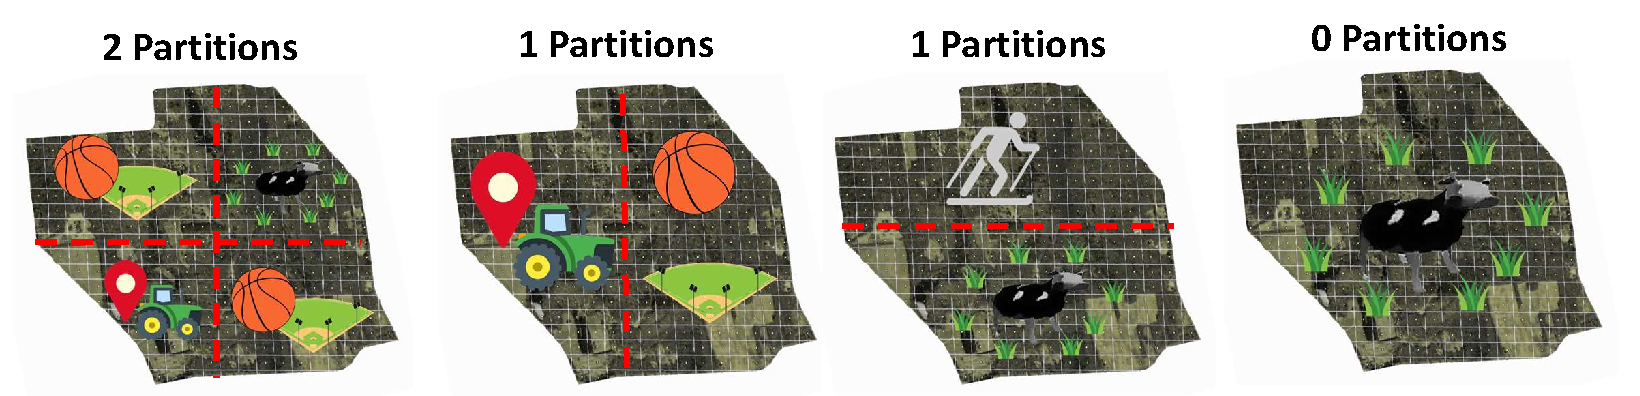
\includegraphics[scale=0.6]{figures/competitorsfigures.pdf}
    \caption{\textbf{Visualization of optimal business choices \textit{after} competitor score revision.}}
    \label{fig:businessnewcompetitorallocations}
\end{figure}

The optimal business choices for the following partitions are listed below. Business allocations that \textit{did change} are italicized. 
\begin{itemize}
    \item \textbf{2 Partitions}: (Top Left) \textbf{\textit{Outdoor Sports Facility}}, (Top Right) \textbf{Grazing Farm}, (Bottom Left) \textbf{\textit{Agritourist Center}}, (Bottom Right) \textbf{Outdoor Sports Complex}.
    \item \textbf{1 Vertical Partition}: (Left) \textbf{\textit{Agritourist Center}}, (Right) \textbf{Outdoor Sports Complex}.
    \item \textbf{1 Horizontal Partition}: (Top) \textbf{\textit{Cross Country Skiing Facility}}, (Bottom) \textbf{\textit{Grazing Area}}.
    \item \textbf{No Partitions}: The optimal business choices is a \textbf{Grazing Area}.
\end{itemize}

It is important to note that some results changed while others stayed the same. This is due to the changing economic factors when we considered the additional company a competitor in our analysis. Additionally, since each business considered the importance of each factor differently (Figure \ref{fig:importancematrix}), the change in economic factors had contrasting effects in our model to better align with each company's values.

\subsubsection{Strengths}

\begin{enumerate} 
   \item This model accounts for both \textbf{negative and positive effects} from company competition.
    \begin{quote}
    When competing companies develop in an area, the hiring market diversifies for local businesses, benefiting both competing and non-competing companies. Our economic model was modified to better account for nearby companies and the associated increase in the employee pool, thus improving the decision process as well. 
    \end{quote}
\end{enumerate}

\subsubsection{Limitations}
\begin{enumerate}
    \item The new competitor score would be \textbf{difficult to measure}.
    \begin{quote}
         As more companies are included in this competitor score, the effect of additional companies on the workforce becomes harder to measure due to the dependent nature of \textit{similar} businesses. Additionally, since many companies form mutualistic relationships with other local companies, it can become difficult to quantify the impact of those relationships on our economic score as the number of relationships increases.
    \end{quote}

    \item The new competitor score does not consider \textbf{competition beyond \textit{similar} industries}.
    \begin{quote}
        Our revised model did not measure adverse effects beyond jobs, such as pollution, community happiness, and overall county economic conditions, which would affect not only \textit{similar} businesses, but also other business options. We decided that the job metric would be the most significant out of these effects, thus we only included the job effects in our model. 
    \end{quote}
\end{enumerate}

\section{Part 4: Generalizability of our Model}
Our model considers numerous parameters, making it possible to customize it to other regions with greater accuracy. By incorporating more relevant information specific to the region, we can better predict the optimal business. As all data used by our model is publicly available, similar information can be obtained for other plots of land.

To analyze other business choices on another plot of land \textbf{both within and outside the United States}, we would require the following data: 

\begin{itemize}
    \item \textbf{Regional data}
    \begin{itemize}
        \item[–] Elevation and detailed topographical data throughout the plot of land.
        \item[–] Previous sunlight data within the new region to predict future sunlight levels.
        \item[–] Historical precipitation data for the region to predict future amounts of precipitation.
        \item[–] Forest coverage percentages throughout the plot of land.
    \end{itemize}
    \item \textbf{Business choice data}
    \begin{itemize}
        \item[–] Economic indicators from \textit{similar} companies for all business choices.
        \item[–] Competitors and their impacts on jobs in the local region of the new region.
    \end{itemize}
\end{itemize}

The business options considered in this model may vary, however, the only \textit{initial} piece of data necessary is the location of the plot of land. All other data and factors can be identified using online sources and geographic information systems, such as ArcGIS. Thus, our model is \textbf{highly versatile} and can be easily adapted to virtually any region of the Earth. 
\newpage
\bibliographystyle{ieeetr}
\bibliography{IM2C}

\pagebreak

\section{Appendices}

\subsection{Appendix 1. Fourier Series Parameters}

\begin{table}[!htbp]
    \begin{tabularx}{\textwidth}{XlXlXlXl}
        \toprule
        \textbf{Parameter} & \textbf{Value} & \textbf{Parameter} & \textbf{Value} \\
        \midrule
        $a_0$ & $-2.17 \cdot 10^1$ & $b_1$ & $-6.79 \cdot 10^0$ \\
        $a_1$ & $4.89 \cdot 10^1$ & $b_2$ & $-1.62 \cdot 10^2$ \\
        $a_2$ & $9.23 \cdot 10^2$ & $b_3$ & $-1.58 \cdot 10^2$ \\
        $a_3$ & $3.24 \cdot 10^1$ & $b_4$ & $3.19 \cdot 10^2$ \\
        $a_4$ & $-9.15 \cdot 10^2$ & $b_5$ & $1.69 \cdot 10^2$ \\
        $a_5$ & $-2.40 \cdot 10^1$ & $b_6$ & $-7.50 \cdot 10^0$ \\
        $a_6$ & $2.37 \cdot 10^1$ & $b_7$ & $1.19 \cdot 10^1$ \\
        $a_7$ & $-2.29 \cdot 10^1$ & $b_8$ & $4.82 \cdot 10^0$ \\
        $a_8$ & $-2.80 \cdot 10^2$ & $b_9$ & $-7.59 \cdot 10^0$ \\
        $a_9$ & $-3.32 \cdot 10^1$ & $b_{10}$ & $-1.05 \cdot 10^2$ \\
        $a_{10}$ & $-2.71 \cdot 10^2$ & $\omega$ & $1.00 \cdot 10^0$ \\
        \bottomrule
    \end{tabularx}
    \caption{\textbf{Fourier parameters and their values.} From Fourier series fitting in Appendix 4.}
    \label{tab:fourierparams}
\end{table}

\newpage 
\subsection{Appendix 2. Collected Financial Data Table}

\begin{table}[!htbp]
\renewcommand{\arraystretch}{1.3}
%p{0.8\linewidth
    \begin{tabularx}{\textwidth}{p{0.1\textwidth} XlXlXlXlXlXl}
   
    \rotatebox{60}{\textbf{Business Model}}           & \rotatebox{60}{\textbf{\textit{Similar}} Company Symbol} & \rotatebox{60}{\textbf{$EBITDA$ Margin}} & \rotatebox{60}{\textbf{$PE$ Ratio}} & \rotatebox{60}{\textbf{Sales Growth}}  & \rotatebox{60}{\textbf{Gross Profit Growth}} 
    & \rotatebox{60}{\textbf{$\sigma$}} & \rotatebox{60}{\textbf{RSI Index}}  & \rotatebox{60}{\textbf{OCF Ratio}} \\ \midrule
    \raggedright   Outdoor Sports Complex & AOUT  & $-0.25$ & $-2.16$ & $40\%$ & $37\%$ & $1.0$ & $52$ & $-0.24$ \\
    \raggedright   Outdoor Sports Complex & DKS  & $0.16$ & $13.17$ & $38.5\%$ & $71.4\%$ & $16$ & $80$ & $1.60$ \\
    \raggedright   Outdoor Sports Complex & ASO  & $0.15$ & $8.58$ & $33.7\%$ & $55.4\%$ & $2$ & $59$ & $1.59$ \\
    \raggedright   Grazing Field & JBSAY  & $0.11$ & $2.37$ & $85.4\%$ & $113\%$ & $0.4$ & $53$ & $1.29$ \\
    \raggedright   Grazing Field & HRL  & $0.13$ & $22.50$ & $30.4\%$ & $34.8\%$ & $5$ & $20$ & $1.03$ \\
    % \raggedright   NONE Agritourist & TRVL  & $--$ & $30.54$ & $-\%$ & $-\%$ & $1$ & $53$ & $1.01$ \\ 
    \raggedright   Ski Resort & MTN  & $0.09$ & $27.11$ & $16\%$ & $9.3\%$ & $6$ & $31$ & $1.095$ \\
    \raggedright   Crop Farm & AGRO  & $0.36$ & $5.40$ & $47.7\%$ & $59.9\%$ & $0.3$ & $42$ & $0.839$ \\
    \raggedright   Crop Farm & FPI  & $0.58$ & $64.44$ & $14.4\%$ & $5.2\%$ & $1.5$ & $25$ & $0.95$ \\
    \raggedright   Regen Farm & GIS  & $0.21$ & $16.46$ & $14.9\%$ &$17.4\%$ & $2$ & $50$ & $1.08$ \\
    \raggedright   Regen Farm & BIMBOA  & $0.15$ & $18.07$ & $35.2\%$ &$32.3\%$ & $2$ & $40$ & $1.54$ \\
    \raggedright   Solar Array & FSLR  & $0.11$ & $40.3$ & $-14.4\%$ &$-87.3\%$ & $45$ & $76$ & $5.01$ \\
    \raggedright   Solar Array & MAXN  & $-0.17$ & $-1.17$ & $-20\%$ &$-330\%$ & $7$ & $76$ & $0.48$ \\
    \raggedright   Agrivoltaic & CUB  & $-9.25$ & $15.68$ & $-20\%$ &$-129.8\%$ & $0.0$ & $52$ & $7.15$ \\
    \raggedright   Agrivoltaic & HFYM  & $-0.57$ & $-3.15$ & $79\%$ &$79\%$ & $0.4$ & $40$ & $0.91$ \\
    
    \bottomrule
    
    \end{tabularx}
    \caption{\textbf{Collected financial data for \textit{similar} companies to business options.}}
    \label{tab:financialdata}
\end{table}

\newpage
\subsection{Appendix 3. ML Sunlight Level Prediction}

\renewcommand{\theFancyVerbLine}{\sffamily\textcolor{gray}{\scriptsize\arabic{FancyVerbLine}\hspace{8pt}}}

\textcolor[rgb]{0.98,0.00,0.00}{\texttt{\textbf{./sunshinepredictor.py}}}
\vspace{0.3em}
\hrule
\inputminted[breaklines, breakanywhere=true, breaksymbolleft=, breaksymbolright=, linenos, numbersep=5pt, xleftmargin=\parindent, style=vs, fontsize=\normalsize]{python}{code/sunshinepredictor.py}

\pagebreak
\subsection{Appendix 4. Fourier Series Precipitation Prediction}

\textcolor[rgb]{0.98,0.00,0.00}{\texttt{\textbf{./fourierregression.py}}}
\vspace{0.3em}
\hrule
\inputminted[breaklines, breakanywhere=true, breaksymbolleft=, breaksymbolright=, linenos, numbersep=5pt, xleftmargin=\parindent, style=vs, fontsize=\normalsize]{python}{./code/sinusodialregression.py}

\pagebreak
\subsection{Appendix 5. (Part 2) Economic Factor Calculation}

\textcolor[rgb]{0.98,0.00,0.00}{\texttt{\textbf{./EconomicalFactorCalculation.py}}}
\vspace{0.3em}
\hrule
\inputminted[breaklines, breaksymbolleft=, breaksymbolright=, linenos, numbersep=5pt, xleftmargin=\parindent, style=vs, fontsize=\normalsize]{python}{./code/economicfactor.py}

\pagebreak
\subsection{Appendix 6. Sliding Windows Implementation}

\textcolor[rgb]{0.98,0.00,0.00}{\texttt{\textbf{./slidingwindows.py}}}
\vspace{0.3em}
\hrule
\inputminted[breaklines, breakanywhere=true, breaksymbolleft=, breaksymbolright=, linenos, numbersep=5pt, xleftmargin=\parindent, style=vs, fontsize=\normalsize]{python}{./code/slidingwindows.py}

\newpage
\subsection{Appendix 7. Importance Matrix Justification}
\begin{figure}[!htbp]
\centering
    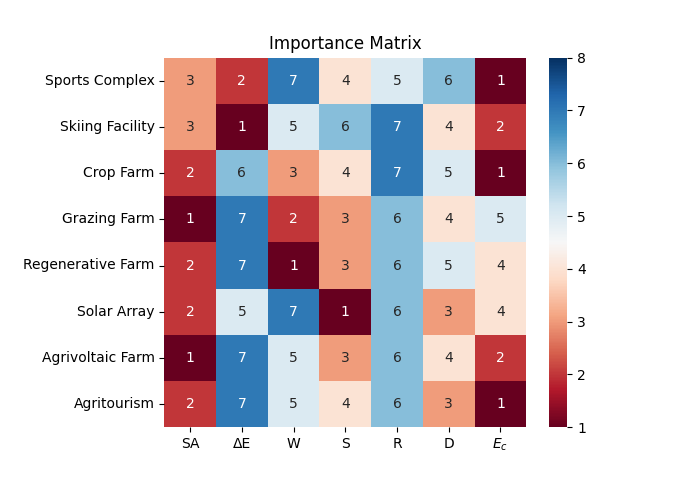
\includegraphics[scale=0.6]{figures/correlationmatrix.png}
\end{figure}

Below we reason more specifically for why we decided to rank each factor for each company.
\begin{itemize}
    \item Sports Complex
    \begin{quote}
        Outdoor sports complexes maintain business by offering recreational fields for people to play sports. Thus, we decided that the economic factor is most important for outdoor sports complexes. Secondly, we decided that elevation and surface area were the following two most important factors because they affect the type and number of fields that can be built on the plot. Next, we determined that sunshine and rain levels are significant factors since outdoor sports usage is affected by weather conditions. Deforestation is a somewhat important but unnecessary factor since it can provide additional space for recreational fields but is not critical. Finally, we ranked proximity to a body of water as the least important factor, as it does not impact the creation or success of an outdoor sports complex.
    \end{quote}

    \item Skiing Facility
    \begin{quote}
        The primary objective of a skiing facility is to offer skiing trails to appeal to snow sports enthusiasts. While economics is critical in sustaining the facility, having skiing trails is essential to attract and retain customers. The most critical factor that affects ski trails is elevation change, ranked first in importance. Economics is ranked second, as it plays a significant role in the facility's sustainability. Usable surface area is also an essential factor, as it determines the length and quantity of ski trails that can be built. We also recognized that deforestation is a crucial factor, as retaining trees on the land enables the creation of more challenging and diverse ski trails. Next, we prioritized proximity to water as the next significant factor, as it can be used for making artificial snow in the ski facility. We ranked sunshine and weather as least important because we are told to assume that there will be sufficient snow coverage. Additionally, skiers do not care about cloud coverage, and skiing is often done at night. 
    \end{quote}

    \item Crop Farm
    \begin{quote} 
       Crop farms primarily grow and harvest crops for sale to food production, making economics the top priority. Usable surface area is the second most important factor, as it directly impacts the number of crops that can be grown. We ranked proximity to a body of water and sunshine levels next in importance because water aids in irrigation, and sunshine aids in crop growth. Deforestation was then ranked as the next important factor since it can clear up additional land for crop growth. However, since only a small fraction of the land is forest, there is already ample space for crop growth. We rated change in elevation as the sixth most important factor because it does not significantly affect the ability to grow crops (e.g., terrace farming can be used). Lastly, rain levels were ranked as a seven because it was previously assumed that there is sufficient irrigation. Being closer to a body of water would be more beneficial than rain because bodies of water also help fertilize crops.
    \end{quote}

    \item Grazing Farm
    \begin{quote}
        The top priority to ensure the success of a grazing farm is to have enough land for raising animals and growing crops to feed them. Thus, the usable surface area is ranked as the most crucial factor. The following important factor is proximity to a body of water, which can serve as a source of water for the animals and provide irrigation to farmland (grass is food for animals). We then rated sunshine levels the next most important factor because they can significantly impact the growth of crops and grass, as well as the ability of animals to be outside and graze.
        We ranked deforestation as the next most crucial factor because deforestation can clear up additional land for grazing animals. Still, it is optional as sufficient land is already available. Because a grazing farm is designed for animals over economics, we ranked economics as the next important factor. The final two factors were rain and change in elevation. These factors were ranked lower because animals will continue to roam regardless of the weather.
    \end{quote}

    \item Regenerative Farm
    \begin{quote}
        Regenerative farms, like crop farms, focus on growing crops, but their emphasis on sustainability and minimum water usage further impacts the factor rankings. We identified the most significant factor as the proximity to a body of water. Regenerative farming emphasizes sustainable practices and minimal water usage. It is located near a body of water and can provide additional irrigation and fertilization, which aligns to use the least possible amount of irrigation necessary. We ranked the usable surface area as the next important factor because having more surface area would allow for the growth of more crops. After that, we determined that sunshine was the third most important factor for crop growth, mainly because a regenerative farm aims to use minimal water. We ranked economics as the next crucial factor since regenerative farms aim to grow crops for the food industry. However, the previously rated factors are essential for achieving that goal. Additionally, we rated deforestation and rainfall as the fifth and sixth most essential factors, respectively, as a regenerative farm has ample land and water access to thrive, making these factors beneficial but not critical. Finally, we deemed a change in elevation the least important factor because different crops require varying elevations to grow. Additionally, we believed that the other factors were more important in determining a business's success than the change in elevation. 
    \end{quote}

    \item Solar Array
    \begin{quote}
        Solar arrays aim to convert sunlight into energy, making sunshine the most crucial factor for their success. We ranked the surface area as the second most important factor for solar arrays since it allows more solar panels to generate more energy. Next, we rated deforestation as the third most important factor since clearing land would create more usable surface area for additional solar panels and more energy production. Next, we considered economics the next most significant factor since the primary goal of a solar farm is to generate energy sustainably for profit. However, the factors rated higher than economics contribute to the business's success and profitability. We ranked the change in elevation and rain levels as the following factors of importance for solar farms, but their impact on the farm's success is relatively less significant. In contrast, a minor change in elevation and lower rain levels may be advantageous, but they are not crucial factors in determining the overall success of the solar farm. Finally, we ranked proximity to a body of water as the least essential factor because being near or far away from a body of water does not affect solar farms or the harvesting of energy in any way.
    \end{quote}

    \item Agrivoltaic Farm
    \begin{quote}
        An agrivoltaic farm is the combination of both a crop farm and a solar array. Because both tasks require large land areas, we ranked the usable surface area as the most critical factor. We determined that economics was the second most crucial factor since, like both crop and solar farms, an agrivoltaic farm aims to generate revenue from the sale of crops and energy. We then assigned sunlight levels as the third most important factor, as it is crucial for the solar panels and beneficial for the crops' growth. We also rated deforestation as the next most crucial factor because an agrivoltaic farm requires solar panels and crop cultivation land, making additional usable land a higher priority. We ranked proximity to a body of water and rain levels as vital factors for agrivoltaic farms. They can play a role in crop growth but do not significantly impact the effectiveness of using solar panels. Lastly, we rated elevation change as the least important factor because, similar to crop and solar farms, the success of an agrivoltaic is least impacted by the change in elevation.
    \end{quote}

    \item Agritourist Center
    \begin{quote}
        The primary focus of an agritourist center is to attract customers through the cultivation of crops and the production of animal products. Therefore, we ranked economics as the most crucial factor. We determined that usable surface area is the second most important factor for an agritourist center because the land will serve multiple purposes, such as crop cultivation, animal raising, visitor building facilities, and selling products. We also considered deforestation the third most important factor due to the benefits of having more usable surface area, as mentioned above. After that, we placed sunshine levels as the fourth most important factor, as it helps crop growth and provides favorable weather for increased tourism. We then considered proximity to a body of water and rain levels as important factors since they contribute to crop growth. However, they are optional, given adequate irrigation. We rated change in elevation as the least important factor because it has a relatively low impact on the success of an agritourist center compared to other factors. Moreover, crops can still be grown on hills, and large tourist buildings can also be built on hills.
    \end{quote}
\end{itemize}

\newpage
\subsection{Appendix 8. (Part 2 and 3) Score and Spearman's Coefficient Calculations}

The following pages in this Appendix are broken up as follows.

\begin{enumerate}
    \item The next 5 pages contain raw score calculations from the decision method for 2, 1, 1, and 0 partitions using the sliding window methodology.

    \item The following 4 pages contain z-score calculations from the raw scores of the previous section. 

    \item The following 4 pages contain High-Low z-score calculations after applying the element-wise multiplication from the \textit{High-Low Matrix}.

    \item The next 16 pages of this Appendix contain the final calculations of the Spearman's Coefficients using ranked z-scores, the importance matrix, and the Spearman's Coefficient formula.

    \item The final 15 pages of this Appendix contain the calculations of Spearman's Rank Correlation Coefficients after applying the revised competitor score. The final page of these contains the Rank Correlation Coefficient scores.

\end{enumerate}

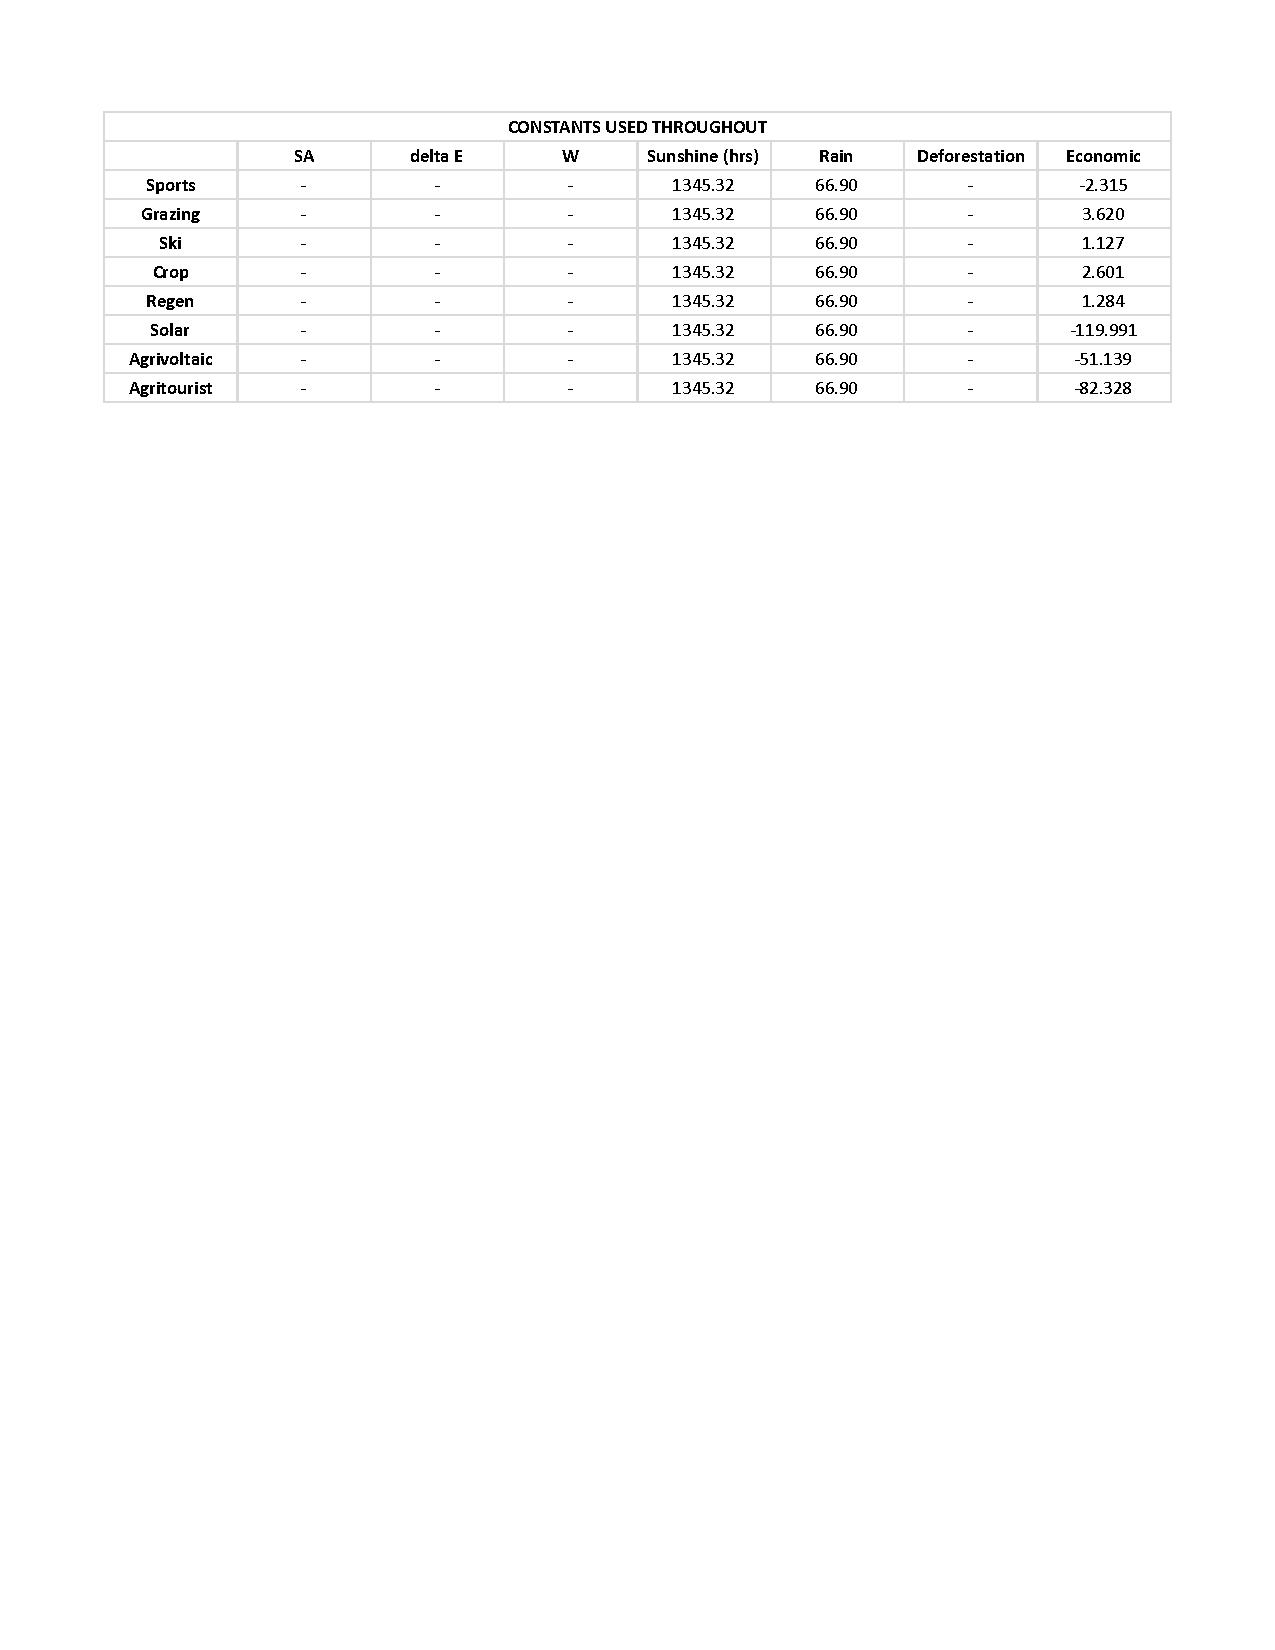
\includepdf[pages=-]{ScoreTables/Raw Scores Table.pdf}

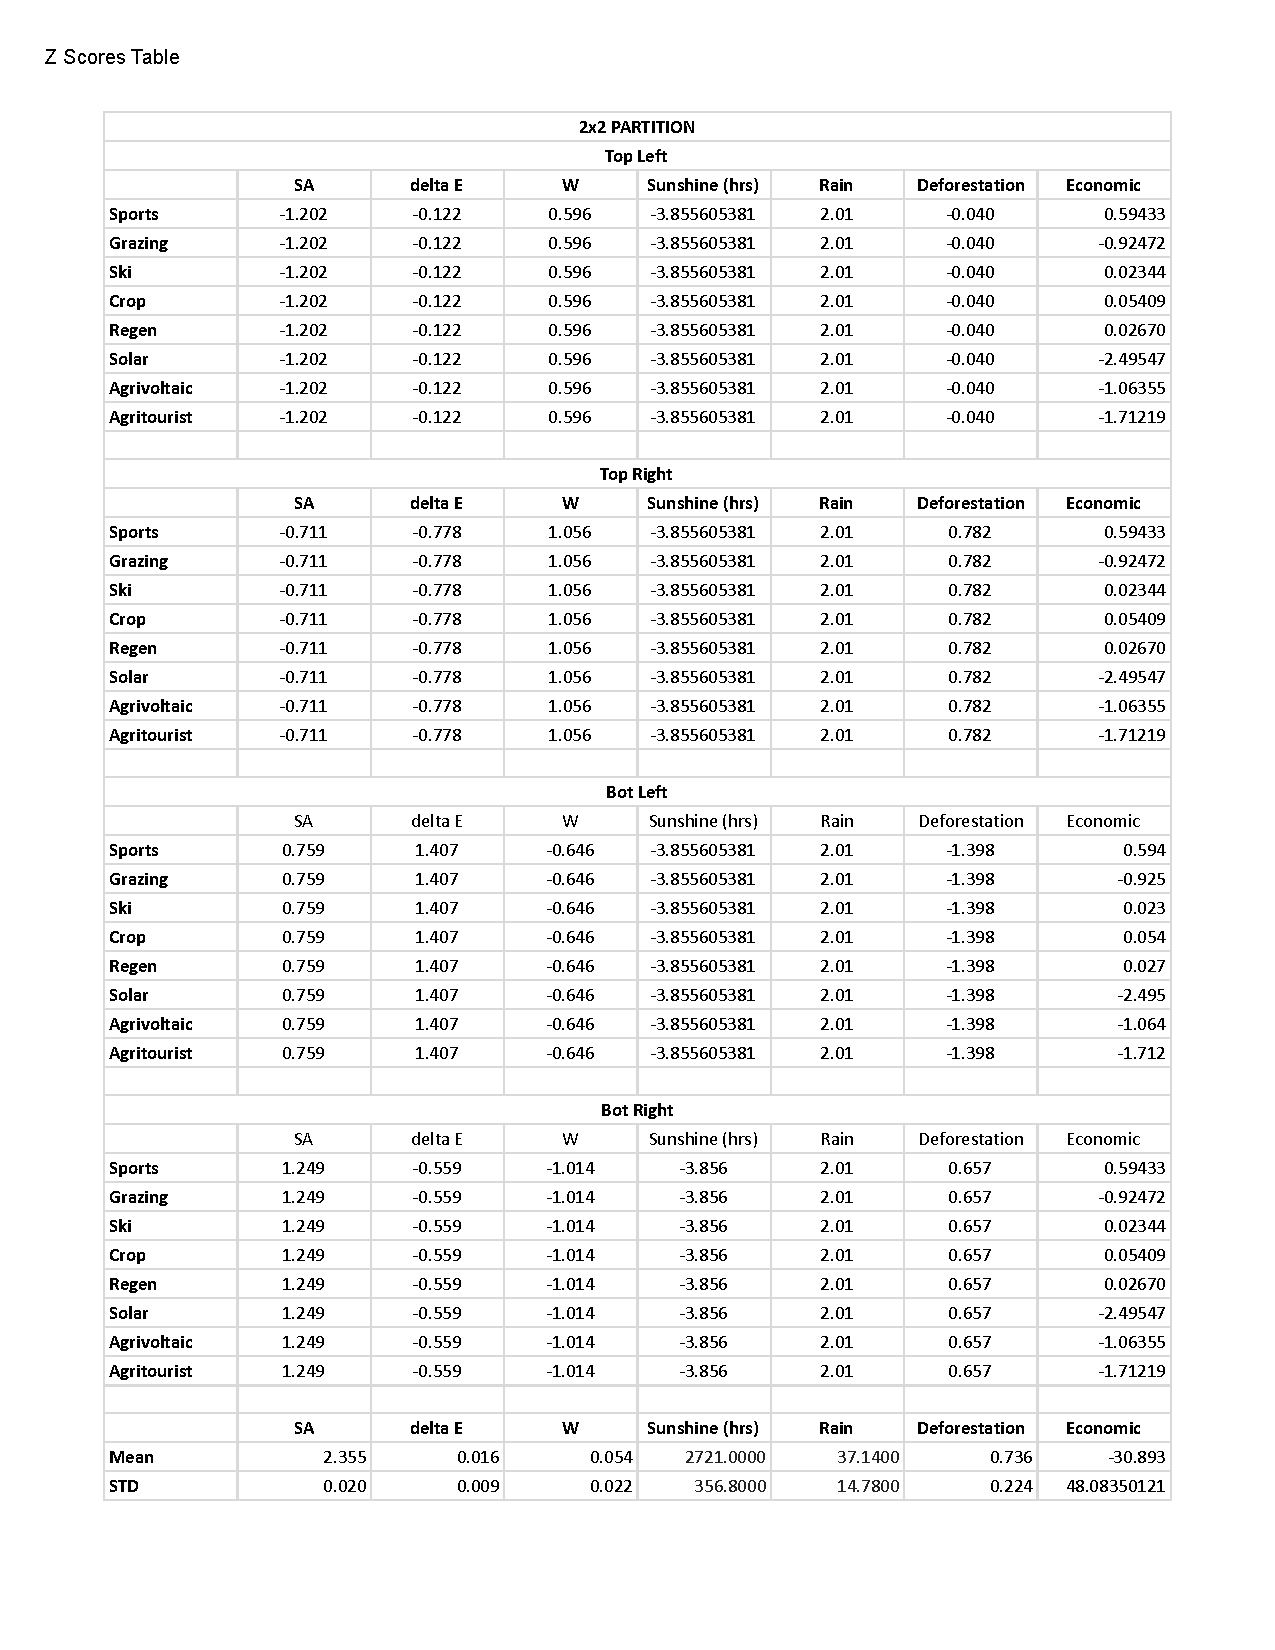
\includepdf[pages=-]{ScoreTables/Z Scores Table.pdf}

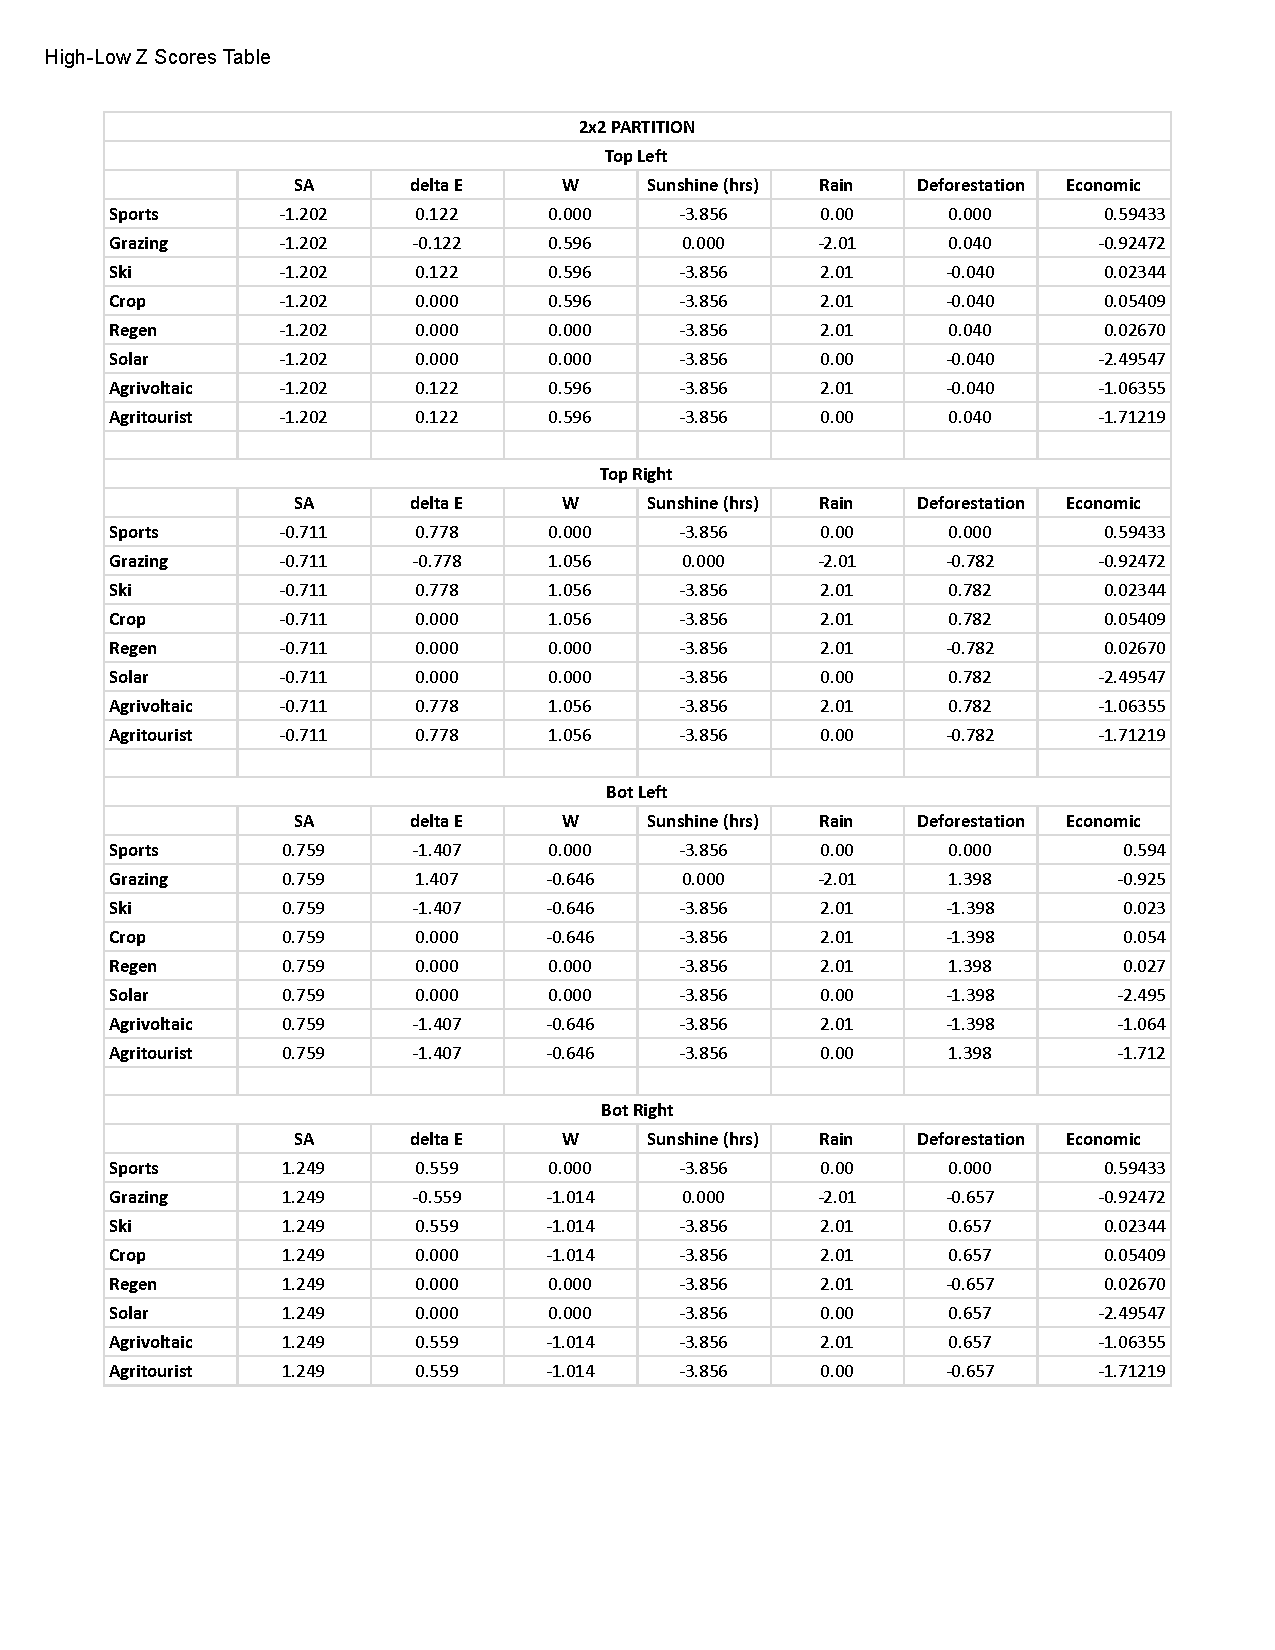
\includepdf[pages=-]{ScoreTables/High-Low Z Scores Table.pdf}

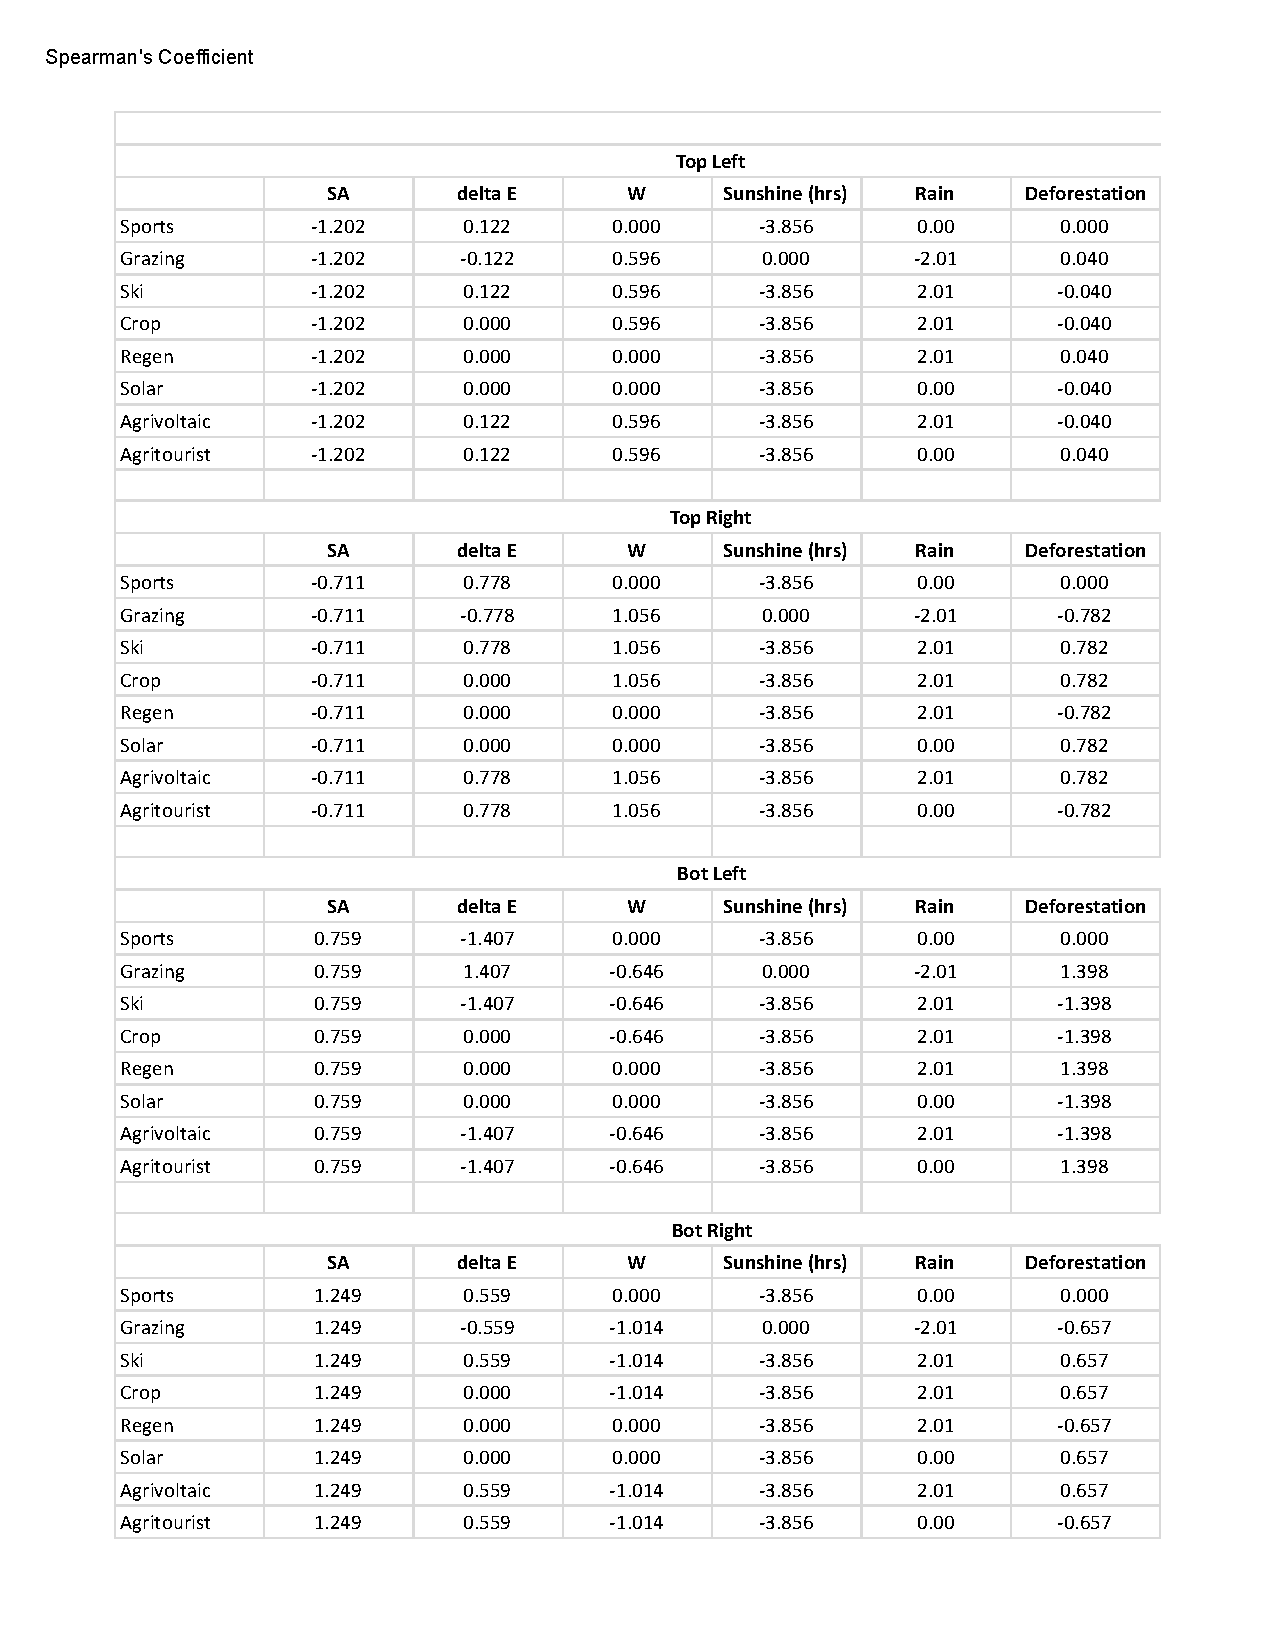
\includepdf[pages=-]{ScoreTables/Spearman's Coefficient.pdf}

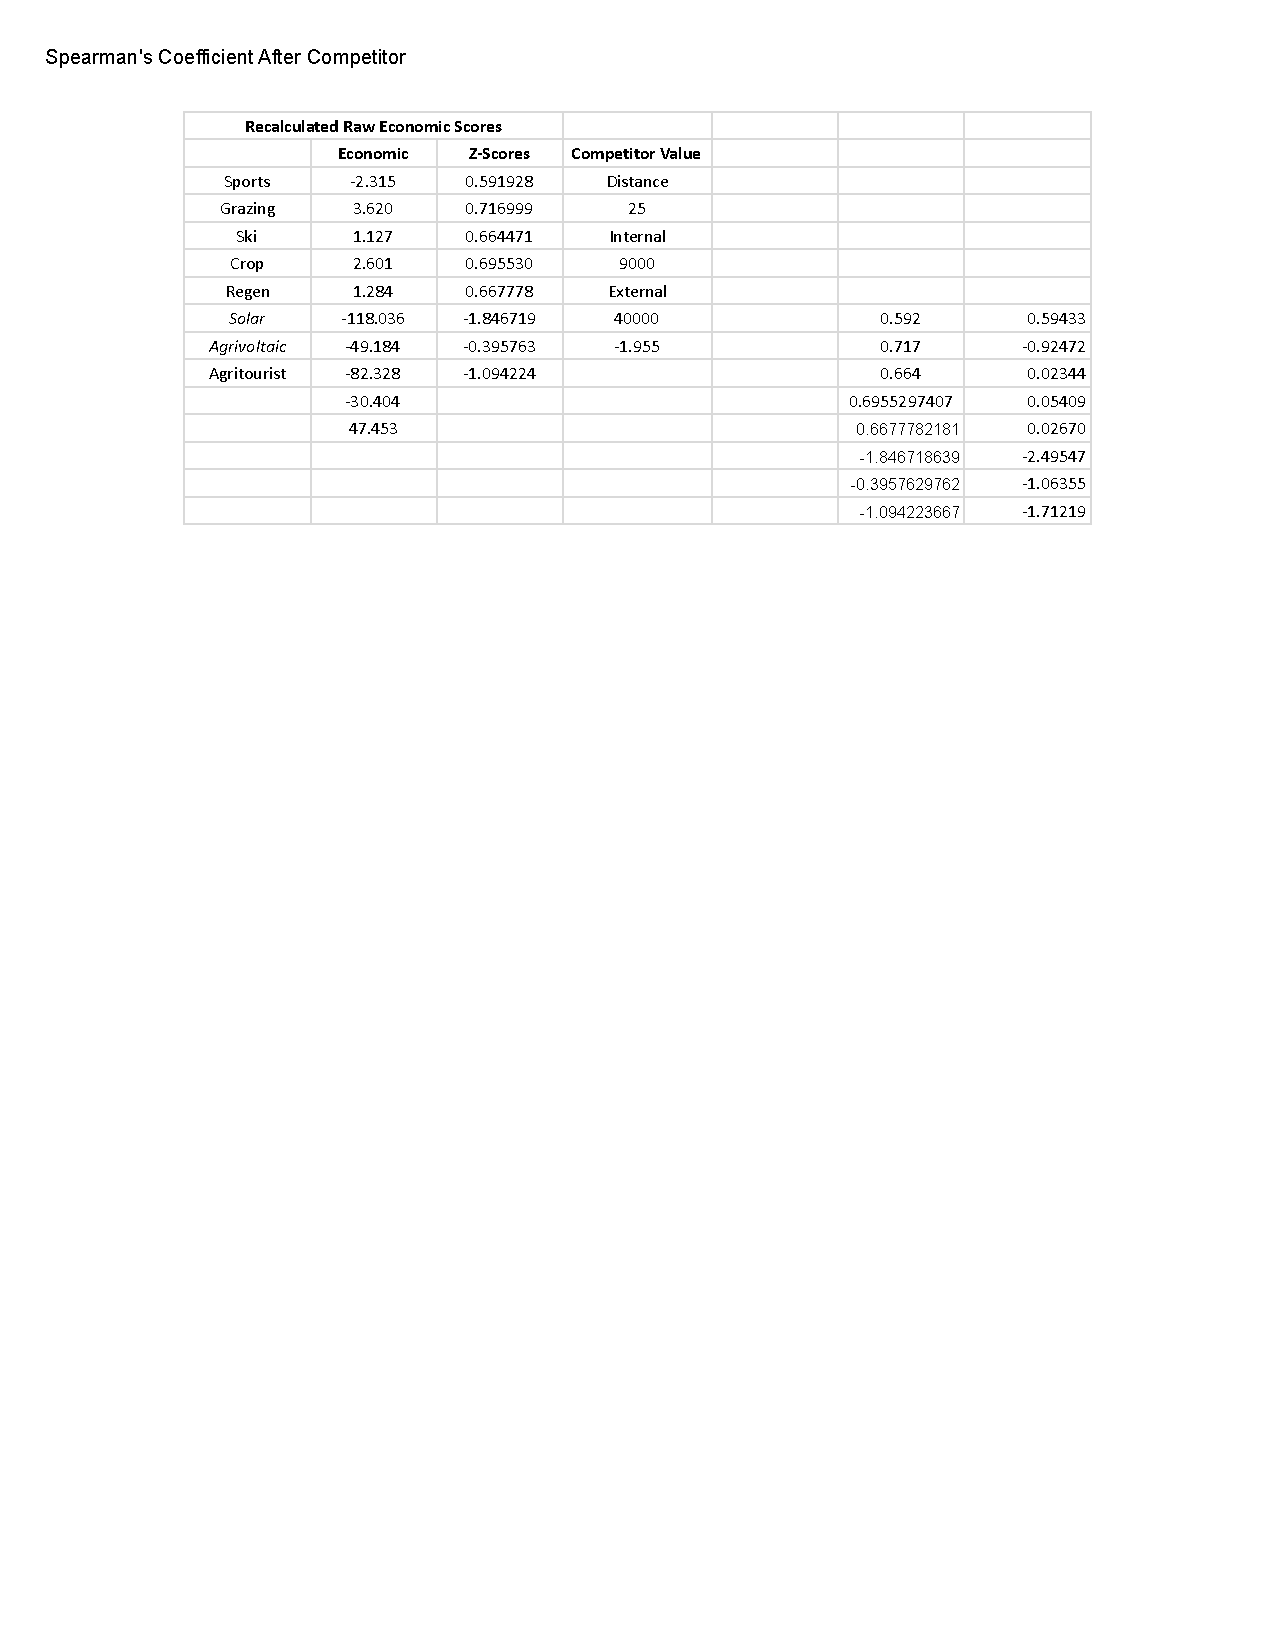
\includepdf[pages=-]{ScoreTables/Spearman's Coefficient After Competitor.pdf}


\end{document}


